\documentclass[12pt,a4paper]{article}
\usepackage[margin=1in,headheight=15pt,headsep=18pt,footskip=30pt]{geometry}
\usepackage{iftex}
\ifPDFTeX
  \usepackage[T1]{fontenc}
  \usepackage[utf8]{inputenc}
  \usepackage{newtxtext}
  \newcommand{\urduword}{Urdu}
\else
  \usepackage{fontspec}
  \setmainfont{Times New Roman}
  \newcommand{\urduword}{Urdu}
\fi
\usepackage[nopatch=footnote]{microtype}
\usepackage{graphicx,float,caption}
\usepackage{chngcntr}
\counterwithin{figure}{section}
\counterwithin{table}{section}
\captionsetup{hypcap=false,font=small,labelsep=space}
\usepackage{longtable,array,pdflscape,etoolbox}
\makeatletter
\patchcmd{\LT@output}{\vss}{\vskip\z@\@plus1fil\@minus\normalbaselineskip}{}{}
\patchcmd{\LT@output}{\vss}{\vskip\z@\@plus1fil\@minus\normalbaselineskip}{}{}
\makeatother
\usepackage{enumitem,setspace,needspace}
\usepackage{fancyhdr}
\usepackage{titlesec}
\usepackage[hidelinks]{hyperref}
\usepackage{xurl}
\usepackage[normalem]{ulem}
\makeatletter
\newcommand{\TocUnderlineEntry}{\@ifnextchar\numberline{\TocUnderlineNumbered}{\TocUnderlineUnnumbered}}
\def\TocUnderlineNumbered\numberline#1#2\TocUnderlineEnd{\numberline{#1}\uline{#2}}
\def\TocUnderlineUnnumbered#1\TocUnderlineEnd{\uline{#1}}
\makeatother
\setlength{\parindent}{0pt}
\setlength{\parskip}{6pt}
\setlength{\emergencystretch}{2em}
\setstretch{1.15}
\setcounter{secnumdepth}{3}
\setcounter{tocdepth}{3}
\titleformat{\section}{\fontsize{14}{17}\selectfont\bfseries}{\thesection.}{0.6em}{}
\titleformat{name=\section,numberless}[block]{\fontsize{14}{17}\selectfont\bfseries}{}{0pt}{}
\titleformat{\subsection}{\fontsize{13}{16}\selectfont\bfseries}{\thesubsection}{0.6em}{}
\titleformat{\subsubsection}{\fontsize{12}{14.4}\selectfont\bfseries}{\thesubsubsection}{0.6em}{}
\titlespacing*{\section}{0pt}{12pt}{6pt}
\titlespacing*{\subsection}{0pt}{10pt}{6pt}
\titlespacing*{\subsubsection}{0pt}{12pt}{8pt}
\renewcommand{\contentsname}{Table of Contents}
\renewcommand{\listfigurename}{LIST OF FIGURES}
\renewcommand{\listtablename}{LIST OF TABLES}
\pagestyle{fancy}
\fancyhf{}
\fancyhead[L]{HomeEase}
\fancyfoot[L]{\small Department of Computer Science, CUI, Abbottabad}
\fancyfoot[R]{\thepage}
\renewcommand{\headrulewidth}{0pt}
\fancypagestyle{frontmatter}{\fancyhf{}\fancyfoot[R]{\thepage}}
\fancypagestyle{thesis}{\fancyhf{}\fancyhead[L]{HomeEase}\fancyfoot[L]{\small Department of Computer Science, CUI, Abbottabad}\fancyfoot[R]{\thepage}}
\begin{document}
\pagestyle{frontmatter}
\pagenumbering{gobble}
\thispagestyle{empty}

\noindent\begin{minipage}[c]{0.24\textwidth}
\centering
\includegraphics[width=1.312in,keepaspectratio]{thesis-assets/image1.jpeg}
\end{minipage}\hfill
\begin{minipage}[c]{0.72\textwidth}
\raggedright\fontsize{14}{18.2}\selectfont\bfseries
COMSATS University Islamabad\\
Abbottabad, Pakistan
\end{minipage}\par

\vspace{12pt}
{\centering\fontsize{18}{23.4}\selectfont\bfseries HomeEase\par}
\vspace{4pt}
{\centering\fontsize{13}{17}\selectfont\bfseries Hyper-Local Domestic Worker Connect Platform with Explainable AI Recommendation \& Bidirectional Marketplace\par}
\vspace{10pt}
{\centering\fontsize{14}{18.2}\selectfont\bfseries\textit{By}\par}
\vspace{8pt}
{\centering\fontsize{13}{17}\selectfont\bfseries Hashir Hamid\hspace*{1.5em}CIIT/FA22-BSE-139/ATD\par}
{\centering\fontsize{13}{17}\selectfont\bfseries Aman Ullah Khan\hspace*{1.5em}CIIT/FA22-BSE-074/ATD\par}
{\centering\fontsize{13}{17}\selectfont\bfseries Umar Saeed\hspace*{1.5em}CIIT/FA22-BCS-041/ATD\par}
\vspace{12pt}
{\centering\fontsize{14}{18.2}\selectfont\bfseries\textit{Supervisor}\\Sir Sumair Khan\par}
\vspace{12pt}
{\centering\fontsize{14}{18.2}\selectfont\bfseries\textit{Bachelor of Science in Computer Science / Software Engineering (2022--2026)}\par}
\vfill
{\centering\fontsize{12}{15.6}\selectfont\bfseries The candidates confirm that the work submitted is their own and appropriate credit has been given where reference has been made to the work of others.\par}

\clearpage
\pagenumbering{roman}
\noindent\begin{minipage}[c]{0.24\textwidth}
\centering
\includegraphics[width=1.312in,keepaspectratio]{thesis-assets/image1.jpeg}
\end{minipage}\hfill
\begin{minipage}[c]{0.72\textwidth}
\raggedright\fontsize{12}{15.6}\selectfont\bfseries
COMSATS University Islamabad, Abbottabad Campus
\end{minipage}\par
\vspace{18pt}
{\centering\fontsize{18}{23.4}\selectfont\bfseries HomeEase\par}
\vspace{14pt}
{\centering\fontsize{14}{18.2}\selectfont\bfseries A project presented to\\COMSATS University Islamabad\par}
\vspace{14pt}
{\centering\fontsize{14}{18.2}\selectfont\bfseries In partial fulfillment of the requirements for the degree of\par}
\vspace{12pt}
{\centering\fontsize{14}{18.2}\selectfont\bfseries\textit{Bachelor of Science in Computer Science / Software Engineering}\\\textit{(2022--2026)}\par}
\vspace{14pt}
{\centering\fontsize{14}{18.2}\selectfont\bfseries By\par}
\vspace{8pt}
{\centering\fontsize{13}{17}\selectfont\bfseries Hashir Hamid\hspace*{1.5em}CIIT/FA22-BSE-139/ATD\par}
{\centering\fontsize{13}{17}\selectfont\bfseries Aman Ullah Khan\hspace*{1.5em}CIIT/FA22-BSE-074/ATD\par}
{\centering\fontsize{13}{17}\selectfont\bfseries Umar Saeed\hspace*{1.5em}CIIT/FA22-BCS-041/ATD\par}

\clearpage
{\centering\bfseries\underline{DECLARATION}\par}
\vspace{8pt}
We hereby declare that this 60\% Final Year Project Thesis Report entitled "HomeEase: Hyper-Local Domestic Worker Connect Platform with Explainable AI Recommendation and Bidirectional Marketplace" is our own original work. No portion of this work has been submitted in support of any other application for another degree or qualification at this or any other university or institute of learning. Appropriate credit, citations, and references have been duly provided wherever external concepts, libraries, frameworks, or standards have been consulted.

The project has been developed under the academic supervision of Sir Sumair Khan at the Department of Computer Science, COMSATS University Islamabad, Abbottabad Campus. The active system adheres strictly to the directives and scope refinements issued by the FYP Evaluation Committee on 2026-09-29, introducing an authentic Content-Based AI recommendation engine, a bidirectional job marketplace, bilingual (Urdu/English) localization, and an Abbottabad cold-start evaluation dataset.

\vspace{28pt}
\noindent
\begin{minipage}[t]{0.31\textwidth}
\centering
Hashir Hamid\\
FA22-BSE-139\\[24pt]
\rule{0.92\linewidth}{0.4pt}\\
Signature
\end{minipage}\hfill
\begin{minipage}[t]{0.31\textwidth}
\centering
Aman Ullah Khan\\
FA22-BSE-074\\[24pt]
\rule{0.92\linewidth}{0.4pt}\\
Signature
\end{minipage}\hfill
\begin{minipage}[t]{0.31\textwidth}
\centering
Umar Saeed\\
FA22-BCS-041\\[24pt]
\rule{0.92\linewidth}{0.4pt}\\
Signature
\end{minipage}

\vspace{34pt}
\begin{center}
Sir Sumair Khan\\
Project Supervisor\\[24pt]
\rule{0.32\linewidth}{0.4pt}\\
Signature
\end{center}
\clearpage
{\centering\bfseries\underline{EXECUTIVE SUMMARY}\par}
\vspace{8pt}
In Pakistan, the domestic informal labor sector—encompassing cooks, cleaners, maids, child nannies, and elderly caregivers—remains largely opaque, decentralized, and governed by informal word-of-mouth networks. This informal hiring paradigm introduces severe friction: households confront safety risks, lack of identity verification, and unpredictable service quality, while domestic workers suffer from arbitrary wage negotiation, undefined task scopes, delayed cash compensations, and lack of professional reputation portability. Furthermore, conventional digital platforms fail in the Pakistani local market because they assume universal English literacy, rely on automated credit card payment gateways that domestic workers cannot access, and employ static database dropdown filters disguised as "recommendations".

To overcome these socio-economic and technical deficits, this project presents HomeEase, a hyper-local domestic worker marketplace designed specifically for local Pakistani dynamics, with primary empirical validation in Abbottabad. HomeEase establishes a structured mobile ecosystem built using Flutter and Dart, backed by Supabase PostgreSQL with Row Level Security (RLS). At this 60\% evaluation milestone, HomeEase successfully fulfills the four official mandates issued by the FYP Evaluation Committee: (1) an authentic Content-Based Vector Similarity Recommender System combining Cosine Similarity on skill feature spaces, Haversine geospatial proximity decay, and min-max rating normalization with Explainable AI (XAI) transparent match badges; (2) a Bidirectional Job Marketplace allowing households to publish open gigs and domestic workers to actively browse and apply for local neighborhood opportunities; (3) a Bilingual Urdu/English localization layer (`EN | \urduword`) with high-affordance visual task icons tailored for low-literacy informal workers; and (4) an Abbottabad synthetic seed dataset and cold-start evaluation benchmark. This document presents the complete 60\% system engineering lifecycle, spanning theoretical foundations, rigorous UML design models, relational schema specifications, algorithmic implementations, and comprehensive verification test suites.

\clearpage
{\centering\bfseries\underline{ACKNOWLEDGEMENT}\par}
\vspace{8pt}
We express our deepest gratitude to Almighty Allah for bestowing upon us the wisdom, health, and perseverance to accomplish this mid-term 60\% software engineering milestone. We extend our sincere appreciation to our project supervisor, Sir Sumair Khan, for his invaluable technical mentorship, constructive critiques, and continuous guidance throughout the architectural design and implementation stages.

We also thank the faculty members of the Department of Computer Science at COMSATS University Islamabad, Abbottabad Campus, for their rigorous evaluation feedback during the 30\% milestone review, which fundamentally elevated the technical depth of this project. Lastly, we owe immense appreciation to our families, fellow students, and our technical mentor AbuZar Babar for their unwavering encouragement, collaborative discussions, and continuous moral support.

\clearpage
{\centering\bfseries\underline{ABBREVIATIONS}\par}
\vspace{8pt}
\begingroup\small\setlength{\tabcolsep}{3pt}\renewcommand{\arraystretch}{1.15}
\begin{longtable}{|>{\raggedright\arraybackslash}p{\dimexpr(\linewidth-4\tabcolsep-3\arrayrulewidth)/2\relax}|>{\raggedright\arraybackslash}p{\dimexpr(\linewidth-4\tabcolsep-3\arrayrulewidth)/2\relax}|}
\hline
\textbf{Abbreviation} & \textbf{Definition} \\ \hline
AI & Artificial Intelligence \\ \hline
BaaS & Backend as a Service \\ \hline
CNIC & Computerized National Identity Card (Pakistan NADRA) \\ \hline
ERD & Entity Relationship Diagram \\ \hline
FK & Foreign Key \\ \hline
HCI & Human-Computer Interaction \\ \hline
JWT & JSON Web Token \\ \hline
KYC & Know Your Customer (Identity \& Background Verification) \\ \hline
PK & Primary Key \\ \hline
REST & Representational State Transfer \\ \hline
RLS & Row Level Security (PostgreSQL) \\ \hline
SDD & Software Design Description \\ \hline
SRS & Software Requirements Specification \\ \hline
XAI & Explainable Artificial Intelligence \\ \hline
\end{longtable}
\endgroup

\clearpage
{\setlength{\parskip}{0pt}\setstretch{1}
\let\OriginalTocContentsLine\contentsline
\renewcommand{\contentsline}[4]{\OriginalTocContentsLine{#1}{\TocUnderlineEntry#2\TocUnderlineEnd}{#3}{#4}}
\tableofcontents
}
\clearpage
{\setlength{\parskip}{0pt}\setstretch{1}\listoffigures}
\clearpage
{\setlength{\parskip}{0pt}\setstretch{1}\listoftables}
\clearpage
\pagenumbering{arabic}
\pagestyle{thesis}
\section{Introduction}
\subsection{Brief Introduction}
HomeEase is an enterprise-grade, hyper-local domestic worker connect platform specifically architected to formalize and secure the informal home-services sector in Pakistan. The platform bridges the deep trust deficit between two primary stakeholders: urban households seeking reliable, safe domestic assistance (such as cooks, cleaners, maids, child nannies, and elderly caregivers), and informal domestic workers who require reliable employment visibility, fair compensation, and professional reputation portability.

In urban and semi-urban Pakistani centers like Abbottabad, domestic worker hiring has historically been restricted to physical word-of-mouth, informal intermediaries, or gatekeeper referrals. These informal channels lack background identity checks, verifiable service histories, transparent task specifications, and standardized wage metrics. Consequently, employers face security risks and unpredictable absenteeism, while domestic workers are exposed to exploitative working hours, arbitrary wage cuts, and zero dispute recourse.

HomeEase establishes a structured digital bridge through a three-tier architecture comprising a Flutter mobile application for both households and workers, a React/Vite admin dashboard for regulatory governance, and a Supabase PostgreSQL backend. At this 60\% evaluation stage, HomeEase extends beyond conventional single-sided directory apps by delivering an Explainable AI (XAI) Recommendation Engine, a Bidirectional Job Marketplace, and a specialized Bilingual/Iconographic accessibility interface tailored for low-literacy workers.

\subsection{Relevance to Course Modules}
The engineering lifecycle and architectural implementation of HomeEase synthesize theoretical knowledge and practical competencies acquired across five core academic modules of the Software Engineering curriculum at COMSATS University Islamabad:

1. CSC392 (Software Engineering): Methodical application of the Agile Scrum methodology, requirement identification techniques, formal SRS and SDD authoring, UML object-oriented modeling, and Software Requirements Traceability Matrices (RTM).

2. CSC341 (Database Systems): Relational database architecture, Third Normal Form (3NF) relational decomposition, entity integrity, foreign key cascading constraints, index optimization, and PostgreSQL Row Level Security (RLS) policies.

3. CSC475 (Artificial Intelligence): Formalization of a Content-Based Recommender System, multi-dimensional feature space vectorization, Cosine Similarity distance metrics in high-dimensional discrete spaces, Haversine spherical distance formulas, min-max normalization, and Explainable AI (XAI) badge synthesis.

4. CSC483 (Mobile Application Development): Cross-platform Flutter architecture, Dart asynchronous programming (Futures, Streams), reactive UI state binding, localized layout constraints, and native hardware sensor integration.

5. CSC412 (Human-Computer Interaction): Usability engineering, accessibility for low-literacy demographics, bilingual right-to-left (RTL) typography handling, and visual iconography affordance design.

\subsection{Project Background}
The HomeEase project commenced with the 10\% Proposal Milestone, identifying the socio-technical breakdown of informal domestic worker hiring in Pakistan. The subsequent 30\% Milestone formulated the complete Software Requirements Specification (SRS v1.0) and Software Design Description (SDD v1.0), along with a 15-screen client-side Flutter prototype executing on an interactive state machine.

During the 60\% evaluation review on 2026-09-29, the FYP Evaluation Committee established four mandatory technical directives: (1) implementing an authentic AI recommendation engine rather than simple SQL filter dropdowns; (2) creating a two-sided bidirectional marketplace enabling workers to search and apply for household gigs; (3) introducing bilingual English/Urdu localization with visual iconography for low-literacy workers; and (4) validating the system with an empirical dataset from Abbottabad. This report documents the successful architectural realization of these mandates.

\subsection{Literature Review}
A rigorous literature review of international and regional on-demand service platforms reveals distinct operational models and limitations:

1. Urban Company (formerly UrbanClap, India/UAE): Employs a full-stack managed marketplace model where the platform sets prices, trains workers, and takes commission. While highly standardized, it requires heavy capital investment, complete digital banking penetration, and excludes informal, low-literacy workers who lack formal trade licenses.

2. Care.com (USA / Global): A subscription-based caregiving directory connecting families with nannies and caregivers. It relies heavily on Social Security Number (SSN) background checks, mandatory monthly credit card subscriptions, and extensive written text profiles, rendering it completely unsuited for the cash-based, low-literacy Pakistani market.

3. Handy \& TaskRabbit (USA / Europe): Gig platforms focusing on handyman tasks, cleaning, and furniture assembly. Both rely on automated credit card escrow and gig-worker bidding. Neither accommodates informal cash settlement, nor do they support visual affordance for workers who cannot read Latin scripts.

4. KaamKaaj \& Local Classifieds (Pakistan / OLX): Local classified platforms simply publish unverified phone numbers and raw text blurbs. They offer zero identity verification, no auto-generated service agreements, no double-booking prevention, no dispute resolution, and zero recommendation intelligence.

\subsection{Analysis from Literature Review}
The reviewed platforms were compared across local matching, worker verification, payment accessibility, marketplace direction, recommendation intelligence, language support, and service agreements.

\begin{itemize}[leftmargin=*,itemsep=6pt]
\item \textbf{Urban Company:} Provides strong worker screening and standardized service terms, but primarily supports card-based payments, platform-assigned work, and text-heavy English/Hindi interfaces.
\item \textbf{Care.com:} Supports caregiver job postings and collaborative recommendations, but relies on credit-card subscriptions, formal identity systems, English content, and does not generate service agreements.
\item \textbf{TaskRabbit:} Offers task feeds, third-party identity checks, and digital escrow, but lacks Urdu support, informal payment handling, and interfaces designed for low-literacy domestic workers.
\item \textbf{Pakistani Classified Platforms:} Support city-level listings and informal cash arrangements, but generally provide no reliable verification, intelligent recommendations, dispute support, payment evidence, or formal agreements.
\item \textbf{HomeEase:} Combines Abbottabad-focused proximity matching, CNIC and police-document verification, Cash/JazzCash/EasyPaisa receipt tracking, a bidirectional job board, explainable content-based recommendations, bilingual English/Urdu interfaces, visual icons, and auto-generated service agreements.
\end{itemize}

\textbf{Critical Research Gap:} No reviewed platform combines hyper-local domestic worker connectivity with explainable AI matching, informal payment auditability, formal service agreements, and bilingual accessibility for low-literacy users in semi-urban Pakistan. HomeEase is designed to address this gap.

\subsection{Methodology and Software Lifecycle for This Project}
HomeEase is developed following the Agile Scrum methodology, organized into two-week development sprints. Agile was selected because domestic worker marketplace workflows require continuous usability testing with both high-literacy employers and low-literacy service providers.

The project lifecycle maps directly to academic milestone checkpoints:

- 10\% Milestone (Proposal): Problem definition, literature review, technical feasibility, and high-level module planning.

- 30\% Milestone (SRS \& SDD): Formal specification of 32 functional requirements, comprehensive UML design suite, 14-table database schema, and client-side Flutter prototype.

- 60\% Milestone (Mid-Term Implementation - Active): Incorporation of the four Committee Mandates: Content-Based AI Recommendation Engine with XAI match badges, Bidirectional Job Marketplace, Bilingual Urdu/English Engine with visual icons, Abbottabad synthetic dataset, and Supabase PostgreSQL integration.

- 100\% Milestone (Final Defense): Live SMS OTP gateway, comprehensive Usability Testing across Abbottabad demographic cohorts, performance benchmarking, and final thesis.

\section{Problem Definition}
\subsection{Problem Statement}
The informal domestic hiring sector in Pakistan suffers from systemic institutional and technological failure, manifested across six core operational pillars:

1. Complete Lack of Background Verification: Households admit domestic workers into private residential spaces with zero verifiable identity records. No centralized repository exists to inspect CNIC authenticity, police character clearance, or past disciplinary histories, creating significant personal and physical security risks.

2. Information Asymmetry and Informal Wage Exploitation: Absence of standardized rate cards leads to arbitrary price gouging by workers or unfair wage depression by employers. Workers lack reputation portability; five years of honest service for one household cannot be digitally proven when seeking employment with another.

3. Single-Sided Friction in Gig Discovery: Traditional platforms treat workers as passive entries in a directory. Workers sitting idle have no mechanism to view nearby households needing immediate assistance, creating severe underemployment.

4. Exclusionary Literacy and Language Barriers: The majority of domestic workers in Pakistan cannot read English, and many have limited Urdu text literacy. Digital platforms built exclusively with dense text menus and complex navigation exclude the very demographic they aim to empower.

5. Cold-Start Failure in Traditional Recommender Systems: Collaborative filtering algorithms rely on millions of historical interaction matrices, causing complete failure during early deployment. Conversely, simple SQL WHERE queries lack algorithmic intelligence and fail academic standards.

6. Unrealistic Digital Payment Gateways: Mandating automated credit card escrow excludes 95\% of domestic workers who operate exclusively in cash or basic mobile wallets (EasyPaisa / JazzCash).

\subsection{Deliverables and Development Requirements}
The HomeEase project delivers a production-style, multi-role domestic-services platform composed of mobile interfaces, an administrative web portal, intelligent matching services, and secure cloud infrastructure. The main deliverables are:

\begin{enumerate}[label=\arabic*.,leftmargin=*,itemsep=7pt]
\item \textbf{Household Mobile Application (Flutter)}\\
A cross-platform mobile experience for household users to register, manage profiles, discover workers, inspect explainable match scores, publish jobs, request bookings, review agreements, record payments, submit reviews, and raise disputes.

\item \textbf{Domestic Worker Mobile Application (Flutter)}\\
A role-specific worker interface for profile creation, service and rate management, availability scheduling, verification-document submission, job browsing, application submission, booking responses, payment confirmation, and reputation tracking.

\item \textbf{Admin Web Dashboard (React, Vite, and TypeScript)}\\
A browser-based governance portal for worker verification, user monitoring, booking and payment audits, dispute handling, evidence review, and basic platform reporting.

\item \textbf{Content-Based Recommendation Engine}\\
An explainable worker-ranking module combining skill-vector cosine similarity, Haversine geographic proximity, and normalized ratings to generate transparent match scores and recommendation badges.

\item \textbf{Bidirectional Job Marketplace}\\
A two-sided marketplace where households publish open service opportunities and verified workers browse and apply for suitable jobs based on category and locality.

\item \textbf{Service Agreement, Payment, and Dispute Modules}\\
Booking-linked agreement generation, manual Cash/JazzCash/EasyPaisa payment evidence, worker payment confirmation, and administrator-mediated dispute resolution.

\item \textbf{Bilingual and Accessible Interface}\\
English/Urdu localization, right-to-left layout support, and high-affordance service icons designed to improve usability for workers with limited English or text literacy.

\item \textbf{Supabase Backend and Abbottabad Dataset}\\
A PostgreSQL database with authentication, Row Level Security, object storage, and a representative Abbottabad seed dataset for development and cold-start recommendation evaluation.
\end{enumerate}

\begingroup\small\setlength{\tabcolsep}{4pt}\renewcommand{\arraystretch}{1.15}
\begin{longtable}{|>{\raggedright\arraybackslash}p{0.22\linewidth}|>{\raggedright\arraybackslash}p{0.29\linewidth}|>{\raggedright\arraybackslash}p{0.41\linewidth}|}
\caption{HomeEase Development Requirements}\label{tab:development-requirements}\\
\hline
\textbf{Category} & \textbf{Requirement} & \textbf{Purpose in HomeEase} \\ \hline
\endfirsthead
\multicolumn{3}{c}{Table \thetable\ HomeEase Development Requirements (continued)}\\
\hline
\textbf{Category} & \textbf{Requirement} & \textbf{Purpose in HomeEase} \\ \hline
\endhead
Mobile Frontend & Flutter SDK 3.x and Dart 3.x & Build household and domestic-worker mobile interfaces for Android and future iOS deployment. \\ \hline
Admin Frontend & React, Vite, TypeScript, and Tailwind CSS & Build the browser-based administration, verification, audit, and dispute-management portal. \\ \hline
Backend Platform & Supabase cloud services & Provide managed authentication, database APIs, storage, and real-time data synchronization. \\ \hline
Database & PostgreSQL 15+ & Store relational records for users, profiles, jobs, bookings, agreements, payments, reviews, and disputes. \\ \hline
Authentication & Supabase Auth and JWT sessions & Secure account access and enforce household, worker, and administrator roles. \\ \hline
Security & PostgreSQL Row Level Security policies & Restrict sensitive profiles, CNIC records, receipts, and dispute evidence to authorized users. \\ \hline
File Storage & Supabase Storage buckets & Store verification documents, payment receipts, profile images, and optional dispute evidence. \\ \hline
Recommendation Logic & Dart/Python vector scoring & Compute explainable skill, location, and rating-based worker recommendations. \\ \hline
Localization & English/Urdu resource dictionaries & Support bilingual content, Urdu rendering, and right-to-left interface behavior. \\ \hline
Development Tools & Android Studio, Visual Studio Code, Git, and GitHub & Support implementation, testing, collaboration, and version control. \\ \hline
Design Tools & Figma and Draw.io/StarUML & Produce user-interface mockups, architecture diagrams, and UML design models. \\ \hline
\end{longtable}
\endgroup
\clearpage\section{Requirement Analysis}
\subsection{System Boundary \& Use Case Diagram}
The HomeEase system boundary encompasses three primary external actors (Household User, Domestic Worker User, and Platform Administrator) interacting with core backend services (Authentication Service, Database Service, AI Recommendation Service, and Notification Service).

Household users execute worker discovery, inspect AI match badges, post open gigs, initiate bookings, sign formal agreements, log manual payments, and file disputes. Domestic workers manage digital profiles, submit KYC documents, set availability calendars, browse open household gigs, submit job proposals, accept bookings, and confirm payment receipts. Administrators govern verification queues, audit transactions, and mediate disputes.

\begin{figure}[H]
\centering
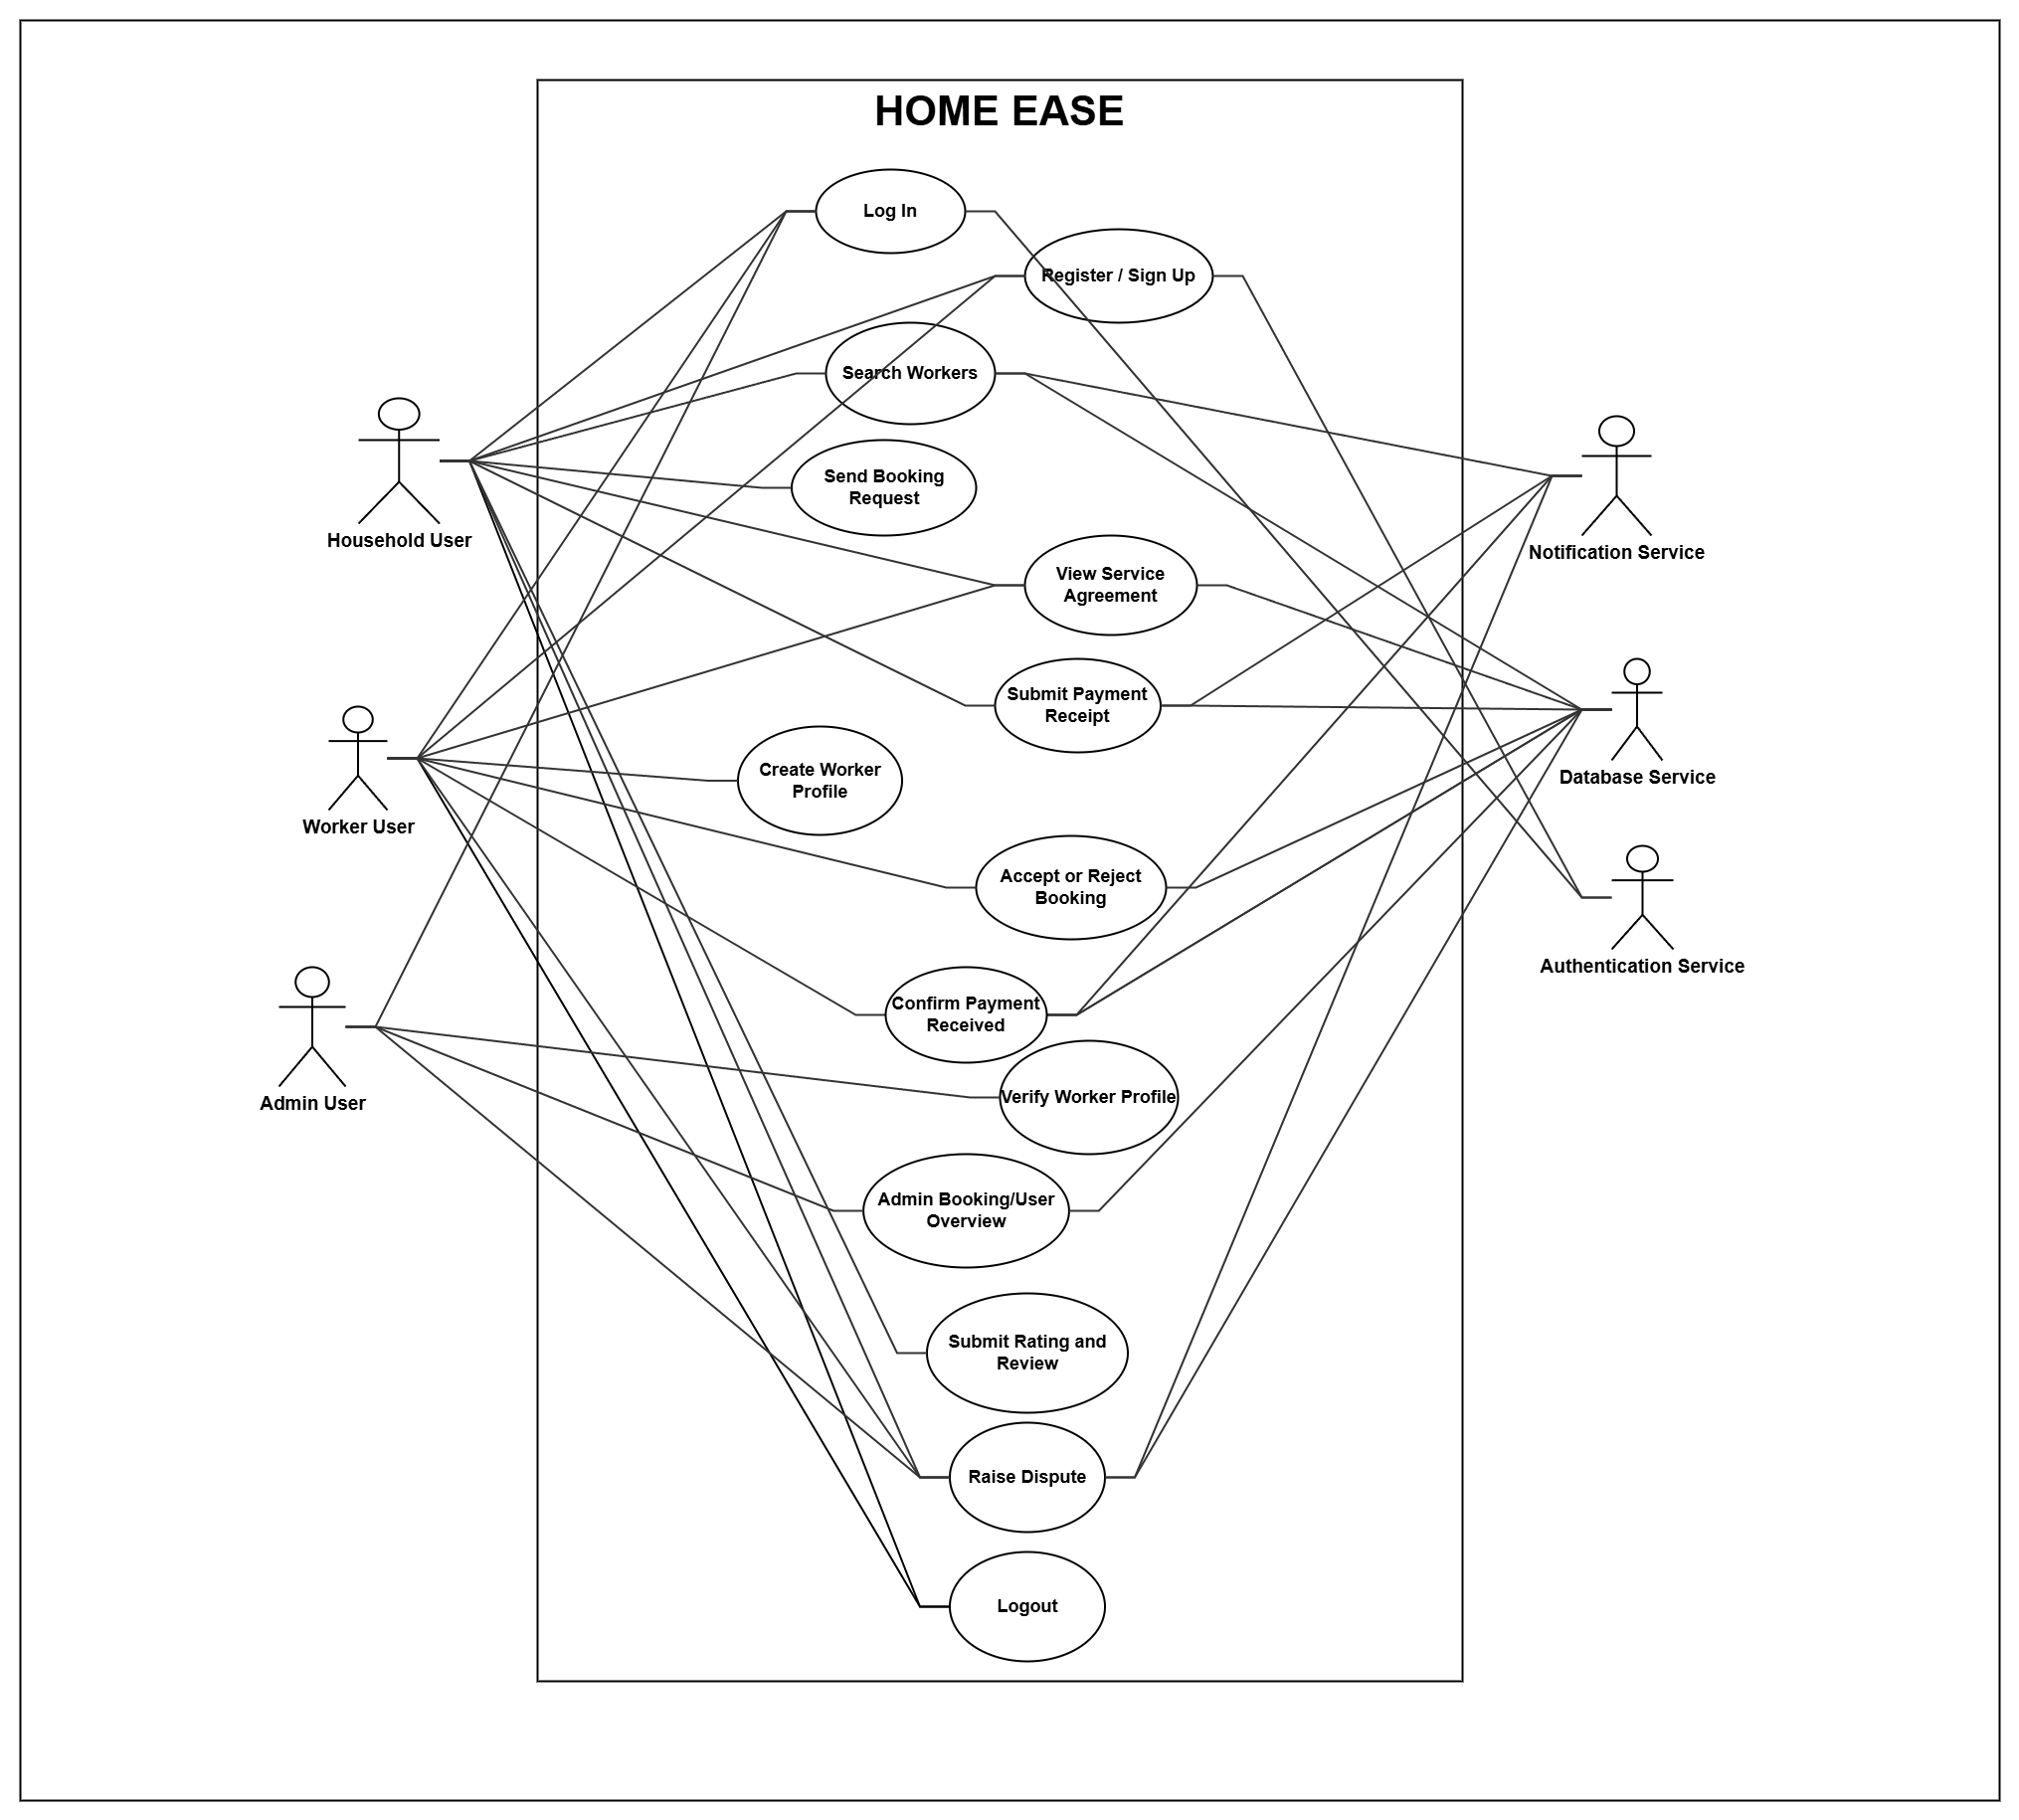
\includegraphics[width=0.95\linewidth,height=0.72\textheight,keepaspectratio]{thesis-assets/image2.png}
\caption{Complete Use Case Diagram for the HomeEase Platform}
\label{fig:use-case}
\end{figure}

\subsection{Detailed Use Cases}
The following use case specifications detail the primary interactions across household, worker, administrative, and algorithmic system actors:

\subsubsection{Household User Use Cases}
\noindent\textbf{UC-HH-01: Household Registration and Profile Setup}\par
\vspace{4pt}
\begingroup\small\setlength{\tabcolsep}{3pt}\renewcommand{\arraystretch}{1.15}
\begin{longtable}{|>{\raggedright\arraybackslash}p{\dimexpr(\linewidth-4\tabcolsep-3\arrayrulewidth)/2\relax}|>{\raggedright\arraybackslash}p{\dimexpr(\linewidth-4\tabcolsep-3\arrayrulewidth)/2\relax}|}
\caption{UC-HH-01: Household Registration and Profile Setup}\label{tab:uc-hh-01}\\
\hline
Specification Field & Detailed System Behavior \\ \hline
Use Case ID & UC-HH-01 \\ \hline
Use Case Name & Household Registration \& Profile Setup \\ \hline
Primary Actor & Household User \\ \hline
Description & A household employer registers a secure account and configures neighborhood location preferences. \\ \hline
Trigger Event & User selects 'Register as Household' on the mobile onboarding screen. \\ \hline
Preconditions & Device has network connectivity. User has a valid mobile number or email. \\ \hline
Postconditions & User account and household profile record are created in Supabase database. \\ \hline
Main Success Flow & 1. User opens app and selects Household role.\newline 2. User enters full name, email/\allowbreak{}phone, password, and Abbottabad locality (e.g., Mandian).\newline 3. System validates credential formats.\newline 4. System creates authentication record and household profile.\newline 5. User is redirected to Household Discovery Home. \\ \hline
\end{longtable}
\endgroup
\clearpage
\noindent\textbf{UC-HH-02: Discover Workers via Content-Based AI Recommender}\par
\vspace{4pt}
\begingroup\small\setlength{\tabcolsep}{3pt}\renewcommand{\arraystretch}{1.15}
\begin{longtable}{|>{\raggedright\arraybackslash}p{\dimexpr(\linewidth-4\tabcolsep-3\arrayrulewidth)/2\relax}|>{\raggedright\arraybackslash}p{\dimexpr(\linewidth-4\tabcolsep-3\arrayrulewidth)/2\relax}|}
\caption{UC-HH-02: Discover Workers via Content-Based AI Recommender}\label{tab:uc-hh-02}\\
\hline
Specification Field & Detailed System Behavior \\ \hline
Use Case ID & UC-HH-02 \\ \hline
Use Case Name & Discover Workers via Content-Based AI Recommender \\ \hline
Primary Actor & Household User \\ \hline
Description & Household views an algorithmically ranked list of domestic workers tailored to service category, geographic proximity, and ratings. \\ \hline
Trigger Event & User opens the HomeEase search hub and selects a service category. \\ \hline
Preconditions & Household location is set. Worker profiles exist in the target region. \\ \hline
Postconditions & System displays sorted worker cards accompanied by Explainable AI (XAI) match percentage badges. \\ \hline
Main Success Flow & 1. Household selects service category (e.g., Cooking).\newline 2. System extracts household feature vector (category, locality coordinates).\newline 3. AI Recommendation Engine computes Cosine similarity, Haversine distance decay, and normalized ratings across active worker profiles.\newline 4. System ranks workers by composite score.\newline 5. UI displays worker cards with match percentage (e.g., '94\% Match') and reasoning tags. \\ \hline
\end{longtable}
\endgroup
\clearpage
\noindent\textbf{UC-HH-03: Publish Open Household Gig or Job Post}\par
\vspace{4pt}
\begingroup\small\setlength{\tabcolsep}{3pt}\renewcommand{\arraystretch}{1.15}
\begin{longtable}{|>{\raggedright\arraybackslash}p{\dimexpr(\linewidth-4\tabcolsep-3\arrayrulewidth)/2\relax}|>{\raggedright\arraybackslash}p{\dimexpr(\linewidth-4\tabcolsep-3\arrayrulewidth)/2\relax}|}
\caption{UC-HH-03: Publish Open Household Gig or Job Post}\label{tab:uc-hh-03}\\
\hline
Specification Field & Detailed System Behavior \\ \hline
Use Case ID & UC-HH-03 \\ \hline
Use Case Name & Publish Open Household Gig / Job Post \\ \hline
Primary Actor & Household User \\ \hline
Description & Household publishes an open domestic task request for local workers to browse and apply (Bidirectional Marketplace). \\ \hline
Trigger Event & Household selects 'Post a Job' from the mobile dashboard. \\ \hline
Preconditions & Household user is authenticated. \\ \hline
Postconditions & New record is created in JOB\_\allowbreak{}POSTS with status 'open' and dispatched to worker feeds. \\ \hline
Main Success Flow & 1. Household enters task title, service category, date/\allowbreak{}time, Abbottabad locality, and proposed budget.\newline 2. User submits the gig posting.\newline 3. System validates inputs and persists job record.\newline 4. Notification service alerts matching domestic workers in the vicinity.\newline 5. Job appears in the Worker 'Available Jobs' feed. \\ \hline
\end{longtable}
\endgroup
\clearpage
\noindent\textbf{UC-HH-04: Direct Booking Request Initiation}\par
\vspace{4pt}
\begingroup\small\setlength{\tabcolsep}{3pt}\renewcommand{\arraystretch}{1.15}
\begin{longtable}{|>{\raggedright\arraybackslash}p{\dimexpr(\linewidth-4\tabcolsep-3\arrayrulewidth)/2\relax}|>{\raggedright\arraybackslash}p{\dimexpr(\linewidth-4\tabcolsep-3\arrayrulewidth)/2\relax}|}
\caption{UC-HH-04: Direct Booking Request Initiation}\label{tab:uc-hh-04}\\
\hline
Specification Field & Detailed System Behavior \\ \hline
Use Case ID & UC-HH-04 \\ \hline
Use Case Name & Direct Booking Request Initiation \\ \hline
Primary Actor & Household User \\ \hline
Description & Household books a specific domestic worker for a defined date, time, and service scope. \\ \hline
Trigger Event & Household taps 'Book Now' on a worker profile screen. \\ \hline
Preconditions & Worker is verified and has open availability slots for the requested date. \\ \hline
Postconditions & Booking record created with status 'Pending'. Double-booking lock engaged. \\ \hline
Main Success Flow & 1. Household selects date, start time, end time, and service tasks.\newline 2. System checks worker availability and verifies no scheduling conflict.\newline 3. Household reviews booking summary and taps 'Send Booking Request'.\newline 4. System creates booking record in BOOKINGS.\newline 5. Notification sent to worker's mobile device. \\ \hline
\end{longtable}
\endgroup
\clearpage
\noindent\textbf{UC-HH-05: Sign Auto-Generated Formal Service Agreement}\par
\vspace{4pt}
\begingroup\small\setlength{\tabcolsep}{3pt}\renewcommand{\arraystretch}{1.15}
\begin{longtable}{|>{\raggedright\arraybackslash}p{\dimexpr(\linewidth-4\tabcolsep-3\arrayrulewidth)/2\relax}|>{\raggedright\arraybackslash}p{\dimexpr(\linewidth-4\tabcolsep-3\arrayrulewidth)/2\relax}|}
\caption{UC-HH-05: Sign Auto-Generated Formal Service Agreement}\label{tab:uc-hh-05}\\
\hline
Specification Field & Detailed System Behavior \\ \hline
Use Case ID & UC-HH-05 \\ \hline
Use Case Name & Sign Auto-Generated Formal Service Agreement \\ \hline
Primary Actor & Household \& Worker \\ \hline
Description & Both parties inspect and digitally sign an auto-generated service contract prior to service commencement. \\ \hline
Trigger Event & Worker accepts a pending booking request. \\ \hline
Preconditions & Booking status is 'Accepted'. \\ \hline
Postconditions & Service agreement record generated in SERVICE\_\allowbreak{}AGREEMENTS with status 'Signed'. \\ \hline
Main Success Flow & 1. System compiles agreed task items, working hours, total wage, locality address, and dispute cancellation policy.\newline 2. Household reviews contract text and clicks 'Agree \& Sign'.\newline 3. Worker reviews contract on their mobile device and clicks 'Confirm Agreement'.\newline 4. Agreement status transitions to 'Active'. \\ \hline
\end{longtable}
\endgroup
\clearpage
\noindent\textbf{UC-HH-06: Log Manual Payment and Upload Receipt}\par
\vspace{4pt}
\begingroup\small\setlength{\tabcolsep}{3pt}\renewcommand{\arraystretch}{1.15}
\begin{longtable}{|>{\raggedright\arraybackslash}p{\dimexpr(\linewidth-4\tabcolsep-3\arrayrulewidth)/2\relax}|>{\raggedright\arraybackslash}p{\dimexpr(\linewidth-4\tabcolsep-3\arrayrulewidth)/2\relax}|}
\caption{UC-HH-06: Log Manual Payment and Upload Receipt}\label{tab:uc-hh-06}\\
\hline
Specification Field & Detailed System Behavior \\ \hline
Use Case ID & UC-HH-06 \\ \hline
Use Case Name & Log Manual Payment \& Upload Receipt \\ \hline
Primary Actor & Household User \\ \hline
Description & Household logs cash or mobile wallet payment (JazzCash/\allowbreak{}EasyPaisa) and uploads receipt proof. \\ \hline
Trigger Event & Service agreement reaches completion date. \\ \hline
Preconditions & Booking status is 'Completed'. \\ \hline
Postconditions & Record created in PAYMENT\_\allowbreak{}RECORDS with status 'Submitted'. Worker notified to confirm. \\ \hline
Main Success Flow & 1. Household selects payment method (Cash, JazzCash, EasyPaisa).\newline 2. Household enters transaction ID / reference and amount paid.\newline 3. User captures image of receipt / screenshot and uploads.\newline 4. System uploads image to Supabase Storage bucket.\newline 5. Notification dispatched to Worker for confirmation. \\ \hline
\end{longtable}
\endgroup
\clearpage
\subsubsection{Domestic Worker Use Cases}
\noindent\textbf{UC-WK-03: Browse Available Jobs Feed}\par
\vspace{4pt}
\begingroup\small\setlength{\tabcolsep}{3pt}\renewcommand{\arraystretch}{1.15}
\begin{longtable}{|>{\raggedright\arraybackslash}p{\dimexpr(\linewidth-4\tabcolsep-3\arrayrulewidth)/2\relax}|>{\raggedright\arraybackslash}p{\dimexpr(\linewidth-4\tabcolsep-3\arrayrulewidth)/2\relax}|}
\caption{UC-WK-03: Browse Available Jobs Feed}\label{tab:uc-wk-03}\\
\hline
Specification Field & Detailed System Behavior \\ \hline
Use Case ID & UC-WK-03 \\ \hline
Use Case Name & Browse Available Jobs Feed (Bidirectional Marketplace) \\ \hline
Primary Actor & Domestic Worker \\ \hline
Description & Worker browses open household job postings matching their trade and location. \\ \hline
Trigger Event & Worker taps 'Find Jobs' tab on the mobile dashboard. \\ \hline
Preconditions & Worker profile has active service categories assigned. \\ \hline
Postconditions & Worker views scrollable list of open gigs with budget, locality, and time requirements. \\ \hline
Main Success Flow & 1. Worker opens 'Available Jobs' feed.\newline 2. System queries JOB\_\allowbreak{}POSTS where status = 'open' matching worker category and locality.\newline 3. Worker inspects job requirements and budget.\newline 4. Worker taps 'Apply Now'.\newline 5. System registers application in JOB\_\allowbreak{}APPLICATIONS and alerts household. \\ \hline
\end{longtable}
\endgroup
\clearpage
\subsubsection{System and General Use Cases}
\noindent\textbf{UC-SYS-01: Content-Based AI Worker Scoring Engine}\par
\vspace{4pt}
\begingroup\small\setlength{\tabcolsep}{3pt}\renewcommand{\arraystretch}{1.15}
\begin{longtable}{|>{\raggedright\arraybackslash}p{\dimexpr(\linewidth-4\tabcolsep-3\arrayrulewidth)/2\relax}|>{\raggedright\arraybackslash}p{\dimexpr(\linewidth-4\tabcolsep-3\arrayrulewidth)/2\relax}|}
\caption{UC-SYS-01: Content-Based AI Worker Scoring Engine}\label{tab:uc-sys-01}\\
\hline
Specification Field & Detailed System Behavior \\ \hline
Use Case ID & UC-SYS-01 \\ \hline
Use Case Name & Content-Based AI Worker Scoring Engine \\ \hline
Primary Actor & System Recommender \\ \hline
Description & Calculates multi-dimensional vector similarity and geographic decay for worker recommendations. \\ \hline
Trigger Event & Household initiates worker search or opens discovery hub. \\ \hline
Preconditions & Household location coordinates and target category vector available. \\ \hline
Postconditions & Normalized match scores and Explainable AI badge strings generated for all candidate workers. \\ \hline
Main Success Flow & 1. System extracts binary category/\allowbreak{}skill vector u for household requirement.\newline 2. System computes Cosine Similarity against worker vectors w\_\allowbreak{}i.\newline 3. System computes Haversine distance d\_\allowbreak{}i in kilometers between household and worker coordinates.\newline 4. System computes proximity decay score S\_\allowbreak{}geo = 1 / (1 + 0.2 d\_\allowbreak{}i).\newline 5. System normalizes worker ratings to [0, 1].\newline 6. System calculates composite score S = 0.50 S\_\allowbreak{}skills + 0.35 S\_\allowbreak{}geo + 0.15 S\_\allowbreak{}rating.\newline 7. System formats explainability string (e.g., '94\% Match \textbullet{} 1.2 km away \textbullet{} Desi Cooking fit'). \\ \hline
\end{longtable}
\endgroup
\clearpage
\noindent\textbf{UC-GEN-01: Bilingual Language and Visual Affordance Toggle}\par
\vspace{4pt}
\begingroup\small\setlength{\tabcolsep}{3pt}\renewcommand{\arraystretch}{1.15}
\begin{longtable}{|>{\raggedright\arraybackslash}p{\dimexpr(\linewidth-4\tabcolsep-3\arrayrulewidth)/2\relax}|>{\raggedright\arraybackslash}p{\dimexpr(\linewidth-4\tabcolsep-3\arrayrulewidth)/2\relax}|}
\caption{UC-GEN-01: Bilingual Language and Visual Affordance Toggle}\label{tab:uc-gen-01}\\
\hline
Specification Field & Detailed System Behavior \\ \hline
Use Case ID & UC-GEN-01 \\ \hline
Use Case Name & Bilingual Language \& Visual Affordance Toggle \\ \hline
Primary Actor & Household \& Worker \\ \hline
Description & User toggles application language between English and Urdu (`\urduword`) with visual icon adaptation. \\ \hline
Trigger Event & User taps the language toggle button (`EN | \urduword`) in the app bar. \\ \hline
Preconditions & Application is running on device. \\ \hline
Postconditions & All screen strings re-render in selected language; RTL direction enabled for Urdu. \\ \hline
Main Success Flow & 1. User clicks language toggle.\newline 2. Localization manager updates active locale state.\newline 3. String resources switch between English and Urdu dictionaries.\newline 4. Layout direction mirrors to Right-To-Left (RTL) for Urdu.\newline 5. Service category cards display high-affordance pictorial icons (Broom, Pot, Stroller, Wheelchair) for immediate visual recognition by low-literacy workers. \\ \hline
\end{longtable}
\endgroup
\clearpage
\subsection{Functional Requirements}
The HomeEase functional requirements are grouped by subsystem. Each requirement is documented separately using the same specification format as the TrekPal reference.

\subsubsection{Authentication Functional Requirements}
Authentication and role-management requirements are as follows.

\Needspace{6\baselineskip}
\noindent\textbf{FR-01: User Account Registration}\par
\vspace{4pt}
\begingroup\small\setlength{\tabcolsep}{4pt}\renewcommand{\arraystretch}{1.15}
\begin{longtable}{|>{\raggedright\arraybackslash}p{0.22\linewidth}|>{\raggedright\arraybackslash}p{0.70\linewidth}|}
\caption{FR-01: User Account Registration}\label{tab:fr-01}\\
\hline
\textbf{Field} & \textbf{Description} \\ \hline
\endfirsthead
\multicolumn{2}{c}{Table \thetable\ User Account Registration (continued)}\\
\hline
\textbf{Field} & \textbf{Description} \\ \hline
\endhead
\textbf{Identifier} & FR-01 \\ \hline
\textbf{Title} & User Account Registration \\ \hline
\textbf{Requirement} & The system shall allow household and worker users to register accounts using email/\allowbreak{}phone and secure password. \\ \hline
\textbf{Source} & Authentication and role-management workflow \\ \hline
\textbf{Rationale} & Required to provide secure, role-appropriate access to HomeEase. \\ \hline
\textbf{Business Rules} & Credentials must be valid and each account must have one authorized role. \\ \hline
\textbf{Dependencies} & Supabase Auth, user profile records, role-based navigation \\ \hline
\textbf{Priority} & High \\ \hline
\end{longtable}
\endgroup

\Needspace{6\baselineskip}
\noindent\textbf{FR-02: Role-Based User Authentication}\par
\vspace{4pt}
\begingroup\small\setlength{\tabcolsep}{4pt}\renewcommand{\arraystretch}{1.15}
\begin{longtable}{|>{\raggedright\arraybackslash}p{0.22\linewidth}|>{\raggedright\arraybackslash}p{0.70\linewidth}|}
\caption{FR-02: Role-Based User Authentication}\label{tab:fr-02}\\
\hline
\textbf{Field} & \textbf{Description} \\ \hline
\endfirsthead
\multicolumn{2}{c}{Table \thetable\ Role-Based User Authentication (continued)}\\
\hline
\textbf{Field} & \textbf{Description} \\ \hline
\endhead
\textbf{Identifier} & FR-02 \\ \hline
\textbf{Title} & Role-Based User Authentication \\ \hline
\textbf{Requirement} & The system shall authenticate registered users and issue role-specific JSON Web Tokens (JWT). \\ \hline
\textbf{Source} & Authentication and role-management workflow \\ \hline
\textbf{Rationale} & Required to provide secure, role-appropriate access to HomeEase. \\ \hline
\textbf{Business Rules} & Credentials must be valid and each account must have one authorized role. \\ \hline
\textbf{Dependencies} & Supabase Auth, user profile records, role-based navigation \\ \hline
\textbf{Priority} & High \\ \hline
\end{longtable}
\endgroup
\clearpage

\Needspace{6\baselineskip}
\noindent\textbf{FR-03: Role Selection and Demo Login}\par
\vspace{4pt}
\begingroup\small\setlength{\tabcolsep}{4pt}\renewcommand{\arraystretch}{1.15}
\begin{longtable}{|>{\raggedright\arraybackslash}p{0.22\linewidth}|>{\raggedright\arraybackslash}p{0.70\linewidth}|}
\caption{FR-03: Role Selection and Demo Login}\label{tab:fr-03}\\
\hline
\textbf{Field} & \textbf{Description} \\ \hline
\endfirsthead
\multicolumn{2}{c}{Table \thetable\ Role Selection and Demo Login (continued)}\\
\hline
\textbf{Field} & \textbf{Description} \\ \hline
\endhead
\textbf{Identifier} & FR-03 \\ \hline
\textbf{Title} & Role Selection and Demo Login \\ \hline
\textbf{Requirement} & The mobile login interface shall allow instant switching and demo credential auto-fill for testing. \\ \hline
\textbf{Source} & Authentication and role-management workflow \\ \hline
\textbf{Rationale} & Required to provide secure, role-appropriate access to HomeEase. \\ \hline
\textbf{Business Rules} & Credentials must be valid and each account must have one authorized role. \\ \hline
\textbf{Dependencies} & Supabase Auth, user profile records, role-based navigation \\ \hline
\textbf{Priority} & Medium \\ \hline
\end{longtable}
\endgroup

\Needspace{6\baselineskip}
\noindent\textbf{FR-04: Role-Based Route Protection}\par
\vspace{4pt}
\begingroup\small\setlength{\tabcolsep}{4pt}\renewcommand{\arraystretch}{1.15}
\begin{longtable}{|>{\raggedright\arraybackslash}p{0.22\linewidth}|>{\raggedright\arraybackslash}p{0.70\linewidth}|}
\caption{FR-04: Role-Based Route Protection}\label{tab:fr-04}\\
\hline
\textbf{Field} & \textbf{Description} \\ \hline
\endfirsthead
\multicolumn{2}{c}{Table \thetable\ Role-Based Route Protection (continued)}\\
\hline
\textbf{Field} & \textbf{Description} \\ \hline
\endhead
\textbf{Identifier} & FR-04 \\ \hline
\textbf{Title} & Role-Based Route Protection \\ \hline
\textbf{Requirement} & The system shall enforce strict role-based route guards preventing unauthorized cross-role access. \\ \hline
\textbf{Source} & Authentication and role-management workflow \\ \hline
\textbf{Rationale} & Required to provide secure, role-appropriate access to HomeEase. \\ \hline
\textbf{Business Rules} & Credentials must be valid and each account must have one authorized role. \\ \hline
\textbf{Dependencies} & Supabase Auth, user profile records, role-based navigation \\ \hline
\textbf{Priority} & High \\ \hline
\end{longtable}
\endgroup
\clearpage

\subsubsection{Household, Worker, and Verification Functional Requirements}
Profile management, worker services, availability, and verification requirements are as follows.

\Needspace{6\baselineskip}
\noindent\textbf{FR-05: Household Profile Management}\par
\vspace{4pt}
\begingroup\small\setlength{\tabcolsep}{4pt}\renewcommand{\arraystretch}{1.15}
\begin{longtable}{|>{\raggedright\arraybackslash}p{0.22\linewidth}|>{\raggedright\arraybackslash}p{0.70\linewidth}|}
\caption{FR-05: Household Profile Management}\label{tab:fr-05}\\
\hline
\textbf{Field} & \textbf{Description} \\ \hline
\endfirsthead
\multicolumn{2}{c}{Table \thetable\ Household Profile Management (continued)}\\
\hline
\textbf{Field} & \textbf{Description} \\ \hline
\endhead
\textbf{Identifier} & FR-05 \\ \hline
\textbf{Title} & Household Profile Management \\ \hline
\textbf{Requirement} & The system shall allow households to manage profile details, contact numbers, and Abbottabad locality address. \\ \hline
\textbf{Source} & UC-HH-01 and household profile workflow \\ \hline
\textbf{Rationale} & Required to store household identity, contact, and service-location information. \\ \hline
\textbf{Business Rules} & Only the authenticated household may update its profile. \\ \hline
\textbf{Dependencies} & Authentication service, household profile table \\ \hline
\textbf{Priority} & High \\ \hline
\end{longtable}
\endgroup

\Needspace{6\baselineskip}
\noindent\textbf{FR-06: Worker Professional Profile Management}\par
\vspace{4pt}
\begingroup\small\setlength{\tabcolsep}{4pt}\renewcommand{\arraystretch}{1.15}
\begin{longtable}{|>{\raggedright\arraybackslash}p{0.22\linewidth}|>{\raggedright\arraybackslash}p{0.70\linewidth}|}
\caption{FR-06: Worker Professional Profile Management}\label{tab:fr-06}\\
\hline
\textbf{Field} & \textbf{Description} \\ \hline
\endfirsthead
\multicolumn{2}{c}{Table \thetable\ Worker Professional Profile Management (continued)}\\
\hline
\textbf{Field} & \textbf{Description} \\ \hline
\endhead
\textbf{Identifier} & FR-06 \\ \hline
\textbf{Title} & Worker Professional Profile Management \\ \hline
\textbf{Requirement} & The system shall allow domestic workers to create professional profiles with bio, experience years, and locality. \\ \hline
\textbf{Source} & Worker profile and service-management workflow \\ \hline
\textbf{Rationale} & Required to present accurate worker skills, pricing, experience, and availability. \\ \hline
\textbf{Business Rules} & Only the profile owner or an authorized administrator may modify worker data. \\ \hline
\textbf{Dependencies} & Worker profile, service category, pricing, and availability records \\ \hline
\textbf{Priority} & High \\ \hline
\end{longtable}
\endgroup
\clearpage

\Needspace{6\baselineskip}
\noindent\textbf{FR-07: Worker Service Category Selection}\par
\vspace{4pt}
\begingroup\small\setlength{\tabcolsep}{4pt}\renewcommand{\arraystretch}{1.15}
\begin{longtable}{|>{\raggedright\arraybackslash}p{0.22\linewidth}|>{\raggedright\arraybackslash}p{0.70\linewidth}|}
\caption{FR-07: Worker Service Category Selection}\label{tab:fr-07}\\
\hline
\textbf{Field} & \textbf{Description} \\ \hline
\endfirsthead
\multicolumn{2}{c}{Table \thetable\ Worker Service Category Selection (continued)}\\
\hline
\textbf{Field} & \textbf{Description} \\ \hline
\endhead
\textbf{Identifier} & FR-07 \\ \hline
\textbf{Title} & Worker Service Category Selection \\ \hline
\textbf{Requirement} & The system shall allow workers to select multiple service categories (Cooking, Cleaning, Childcare, Elderly Care). \\ \hline
\textbf{Source} & Worker profile and service-management workflow \\ \hline
\textbf{Rationale} & Required to present accurate worker skills, pricing, experience, and availability. \\ \hline
\textbf{Business Rules} & Only the profile owner or an authorized administrator may modify worker data. \\ \hline
\textbf{Dependencies} & Worker profile, service category, pricing, and availability records \\ \hline
\textbf{Priority} & High \\ \hline
\end{longtable}
\endgroup

\Needspace{6\baselineskip}
\noindent\textbf{FR-08: Worker Service Rate Configuration}\par
\vspace{4pt}
\begingroup\small\setlength{\tabcolsep}{4pt}\renewcommand{\arraystretch}{1.15}
\begin{longtable}{|>{\raggedright\arraybackslash}p{0.22\linewidth}|>{\raggedright\arraybackslash}p{0.70\linewidth}|}
\caption{FR-08: Worker Service Rate Configuration}\label{tab:fr-08}\\
\hline
\textbf{Field} & \textbf{Description} \\ \hline
\endfirsthead
\multicolumn{2}{c}{Table \thetable\ Worker Service Rate Configuration (continued)}\\
\hline
\textbf{Field} & \textbf{Description} \\ \hline
\endhead
\textbf{Identifier} & FR-08 \\ \hline
\textbf{Title} & Worker Service Rate Configuration \\ \hline
\textbf{Requirement} & The system shall allow workers to configure hourly or visit-based charge rates per service category. \\ \hline
\textbf{Source} & Worker profile and service-management workflow \\ \hline
\textbf{Rationale} & Required to present accurate worker skills, pricing, experience, and availability. \\ \hline
\textbf{Business Rules} & Only the profile owner or an authorized administrator may modify worker data. \\ \hline
\textbf{Dependencies} & Worker profile, service category, pricing, and availability records \\ \hline
\textbf{Priority} & Medium \\ \hline
\end{longtable}
\endgroup
\clearpage

\Needspace{6\baselineskip}
\noindent\textbf{FR-09: Worker Availability Scheduling}\par
\vspace{4pt}
\begingroup\small\setlength{\tabcolsep}{4pt}\renewcommand{\arraystretch}{1.15}
\begin{longtable}{|>{\raggedright\arraybackslash}p{0.22\linewidth}|>{\raggedright\arraybackslash}p{0.70\linewidth}|}
\caption{FR-09: Worker Availability Scheduling}\label{tab:fr-09}\\
\hline
\textbf{Field} & \textbf{Description} \\ \hline
\endfirsthead
\multicolumn{2}{c}{Table \thetable\ Worker Availability Scheduling (continued)}\\
\hline
\textbf{Field} & \textbf{Description} \\ \hline
\endhead
\textbf{Identifier} & FR-09 \\ \hline
\textbf{Title} & Worker Availability Scheduling \\ \hline
\textbf{Requirement} & The system shall provide a weekly calendar allowing workers to toggle availability time slots by day of week. \\ \hline
\textbf{Source} & Worker profile and service-management workflow \\ \hline
\textbf{Rationale} & Required to present accurate worker skills, pricing, experience, and availability. \\ \hline
\textbf{Business Rules} & Only the profile owner or an authorized administrator may modify worker data. \\ \hline
\textbf{Dependencies} & Worker profile, service category, pricing, and availability records \\ \hline
\textbf{Priority} & High \\ \hline
\end{longtable}
\endgroup

\Needspace{6\baselineskip}
\noindent\textbf{FR-10: Worker Verification Document Submission}\par
\vspace{4pt}
\begingroup\small\setlength{\tabcolsep}{4pt}\renewcommand{\arraystretch}{1.15}
\begin{longtable}{|>{\raggedright\arraybackslash}p{0.22\linewidth}|>{\raggedright\arraybackslash}p{0.70\linewidth}|}
\caption{FR-10: Worker Verification Document Submission}\label{tab:fr-10}\\
\hline
\textbf{Field} & \textbf{Description} \\ \hline
\endfirsthead
\multicolumn{2}{c}{Table \thetable\ Worker Verification Document Submission (continued)}\\
\hline
\textbf{Field} & \textbf{Description} \\ \hline
\endhead
\textbf{Identifier} & FR-10 \\ \hline
\textbf{Title} & Worker Verification Document Submission \\ \hline
\textbf{Requirement} & The system shall allow workers to upload CNIC front/\allowbreak{}back images and character certificates for verification. \\ \hline
\textbf{Source} & Worker verification workflow \\ \hline
\textbf{Rationale} & Required to establish worker identity and platform trust. \\ \hline
\textbf{Business Rules} & Required documents must be complete before administrative review. \\ \hline
\textbf{Dependencies} & Worker profile, secure storage, admin verification queue \\ \hline
\textbf{Priority} & High \\ \hline
\end{longtable}
\endgroup
\clearpage

\subsubsection{Recommendation and Job Marketplace Functional Requirements}
AI matching and bidirectional job-marketplace requirements are as follows.

\Needspace{6\baselineskip}
\noindent\textbf{FR-11: Skill Vector Generation}\par
\vspace{4pt}
\begingroup\small\setlength{\tabcolsep}{4pt}\renewcommand{\arraystretch}{1.15}
\begin{longtable}{|>{\raggedright\arraybackslash}p{0.22\linewidth}|>{\raggedright\arraybackslash}p{0.70\linewidth}|}
\caption{FR-11: Skill Vector Generation}\label{tab:fr-11}\\
\hline
\textbf{Field} & \textbf{Description} \\ \hline
\endfirsthead
\multicolumn{2}{c}{Table \thetable\ Skill Vector Generation (continued)}\\
\hline
\textbf{Field} & \textbf{Description} \\ \hline
\endhead
\textbf{Identifier} & FR-11 \\ \hline
\textbf{Title} & Skill Vector Generation \\ \hline
\textbf{Requirement} & The system shall vectorize household requirements and compute Content-Based Cosine Similarity on worker skills. \\ \hline
\textbf{Source} & UC-SYS-01 Content-Based AI Worker Scoring Engine \\ \hline
\textbf{Rationale} & Required to rank suitable workers transparently for household users. \\ \hline
\textbf{Business Rules} & Scores must use available skill, location, and rating data without hidden manual ordering. \\ \hline
\textbf{Dependencies} & Worker services, household requirements, coordinates, ratings \\ \hline
\textbf{Priority} & High \\ \hline
\end{longtable}
\endgroup

\Needspace{6\baselineskip}
\noindent\textbf{FR-12: Geographic Distance Calculation}\par
\vspace{4pt}
\begingroup\small\setlength{\tabcolsep}{4pt}\renewcommand{\arraystretch}{1.15}
\begin{longtable}{|>{\raggedright\arraybackslash}p{0.22\linewidth}|>{\raggedright\arraybackslash}p{0.70\linewidth}|}
\caption{FR-12: Geographic Distance Calculation}\label{tab:fr-12}\\
\hline
\textbf{Field} & \textbf{Description} \\ \hline
\endfirsthead
\multicolumn{2}{c}{Table \thetable\ Geographic Distance Calculation (continued)}\\
\hline
\textbf{Field} & \textbf{Description} \\ \hline
\endhead
\textbf{Identifier} & FR-12 \\ \hline
\textbf{Title} & Geographic Distance Calculation \\ \hline
\textbf{Requirement} & The system shall calculate Haversine geographic distance between household and worker coordinates. \\ \hline
\textbf{Source} & UC-SYS-01 Content-Based AI Worker Scoring Engine \\ \hline
\textbf{Rationale} & Required to rank suitable workers transparently for household users. \\ \hline
\textbf{Business Rules} & Scores must use available skill, location, and rating data without hidden manual ordering. \\ \hline
\textbf{Dependencies} & Worker services, household requirements, coordinates, ratings \\ \hline
\textbf{Priority} & High \\ \hline
\end{longtable}
\endgroup
\clearpage

\Needspace{6\baselineskip}
\noindent\textbf{FR-13: Explainable Composite Match Scoring}\par
\vspace{4pt}
\begingroup\small\setlength{\tabcolsep}{4pt}\renewcommand{\arraystretch}{1.15}
\begin{longtable}{|>{\raggedright\arraybackslash}p{0.22\linewidth}|>{\raggedright\arraybackslash}p{0.70\linewidth}|}
\caption{FR-13: Explainable Composite Match Scoring}\label{tab:fr-13}\\
\hline
\textbf{Field} & \textbf{Description} \\ \hline
\endfirsthead
\multicolumn{2}{c}{Table \thetable\ Explainable Composite Match Scoring (continued)}\\
\hline
\textbf{Field} & \textbf{Description} \\ \hline
\endhead
\textbf{Identifier} & FR-13 \\ \hline
\textbf{Title} & Explainable Composite Match Scoring \\ \hline
\textbf{Requirement} & The system shall compute a composite recommendation match score and display transparent Explainable AI badges. \\ \hline
\textbf{Source} & UC-SYS-01 Content-Based AI Worker Scoring Engine \\ \hline
\textbf{Rationale} & Required to rank suitable workers transparently for household users. \\ \hline
\textbf{Business Rules} & Scores must use available skill, location, and rating data without hidden manual ordering. \\ \hline
\textbf{Dependencies} & Worker services, household requirements, coordinates, ratings \\ \hline
\textbf{Priority} & High \\ \hline
\end{longtable}
\endgroup

\Needspace{6\baselineskip}
\noindent\textbf{FR-14: Household Job Post Creation}\par
\vspace{4pt}
\begingroup\small\setlength{\tabcolsep}{4pt}\renewcommand{\arraystretch}{1.15}
\begin{longtable}{|>{\raggedright\arraybackslash}p{0.22\linewidth}|>{\raggedright\arraybackslash}p{0.70\linewidth}|}
\caption{FR-14: Household Job Post Creation}\label{tab:fr-14}\\
\hline
\textbf{Field} & \textbf{Description} \\ \hline
\endfirsthead
\multicolumn{2}{c}{Table \thetable\ Household Job Post Creation (continued)}\\
\hline
\textbf{Field} & \textbf{Description} \\ \hline
\endhead
\textbf{Identifier} & FR-14 \\ \hline
\textbf{Title} & Household Job Post Creation \\ \hline
\textbf{Requirement} & The system shall allow households to publish open domestic job postings with category, budget, date, and locality. \\ \hline
\textbf{Source} & UC-HH-03 and UC-WK-03 \\ \hline
\textbf{Rationale} & Required to support a bidirectional marketplace where households post jobs and workers apply. \\ \hline
\textbf{Business Rules} & Only open jobs may appear in worker feeds or accept applications. \\ \hline
\textbf{Dependencies} & Job posts, job applications, profiles, notification service \\ \hline
\textbf{Priority} & High \\ \hline
\end{longtable}
\endgroup
\clearpage

\Needspace{6\baselineskip}
\noindent\textbf{FR-15: Worker Job Feed}\par
\vspace{4pt}
\begingroup\small\setlength{\tabcolsep}{4pt}\renewcommand{\arraystretch}{1.15}
\begin{longtable}{|>{\raggedright\arraybackslash}p{0.22\linewidth}|>{\raggedright\arraybackslash}p{0.70\linewidth}|}
\caption{FR-15: Worker Job Feed}\label{tab:fr-15}\\
\hline
\textbf{Field} & \textbf{Description} \\ \hline
\endfirsthead
\multicolumn{2}{c}{Table \thetable\ Worker Job Feed (continued)}\\
\hline
\textbf{Field} & \textbf{Description} \\ \hline
\endhead
\textbf{Identifier} & FR-15 \\ \hline
\textbf{Title} & Worker Job Feed \\ \hline
\textbf{Requirement} & The system shall display a live feed of open household gigs to domestic workers matching their category and locality. \\ \hline
\textbf{Source} & UC-HH-03 and UC-WK-03 \\ \hline
\textbf{Rationale} & Required to support a bidirectional marketplace where households post jobs and workers apply. \\ \hline
\textbf{Business Rules} & Only open jobs may appear in worker feeds or accept applications. \\ \hline
\textbf{Dependencies} & Job posts, job applications, profiles, notification service \\ \hline
\textbf{Priority} & High \\ \hline
\end{longtable}
\endgroup

\Needspace{6\baselineskip}
\noindent\textbf{FR-16: Worker Job Application}\par
\vspace{4pt}
\begingroup\small\setlength{\tabcolsep}{4pt}\renewcommand{\arraystretch}{1.15}
\begin{longtable}{|>{\raggedright\arraybackslash}p{0.22\linewidth}|>{\raggedright\arraybackslash}p{0.70\linewidth}|}
\caption{FR-16: Worker Job Application}\label{tab:fr-16}\\
\hline
\textbf{Field} & \textbf{Description} \\ \hline
\endfirsthead
\multicolumn{2}{c}{Table \thetable\ Worker Job Application (continued)}\\
\hline
\textbf{Field} & \textbf{Description} \\ \hline
\endhead
\textbf{Identifier} & FR-16 \\ \hline
\textbf{Title} & Worker Job Application \\ \hline
\textbf{Requirement} & The system shall allow domestic workers to apply to open household job postings with a single tap. \\ \hline
\textbf{Source} & UC-HH-03 and UC-WK-03 \\ \hline
\textbf{Rationale} & Required to support a bidirectional marketplace where households post jobs and workers apply. \\ \hline
\textbf{Business Rules} & Only open jobs may appear in worker feeds or accept applications. \\ \hline
\textbf{Dependencies} & Job posts, job applications, profiles, notification service \\ \hline
\textbf{Priority} & High \\ \hline
\end{longtable}
\endgroup
\clearpage

\Needspace{6\baselineskip}
\noindent\textbf{FR-17: Household Job Application Notification}\par
\vspace{4pt}
\begingroup\small\setlength{\tabcolsep}{4pt}\renewcommand{\arraystretch}{1.15}
\begin{longtable}{|>{\raggedright\arraybackslash}p{0.22\linewidth}|>{\raggedright\arraybackslash}p{0.70\linewidth}|}
\caption{FR-17: Household Job Application Notification}\label{tab:fr-17}\\
\hline
\textbf{Field} & \textbf{Description} \\ \hline
\endfirsthead
\multicolumn{2}{c}{Table \thetable\ Household Job Application Notification (continued)}\\
\hline
\textbf{Field} & \textbf{Description} \\ \hline
\endhead
\textbf{Identifier} & FR-17 \\ \hline
\textbf{Title} & Household Job Application Notification \\ \hline
\textbf{Requirement} & The system shall notify households immediately upon receiving worker job applications. \\ \hline
\textbf{Source} & UC-HH-03 and UC-WK-03 \\ \hline
\textbf{Rationale} & Required to support a bidirectional marketplace where households post jobs and workers apply. \\ \hline
\textbf{Business Rules} & Only open jobs may appear in worker feeds or accept applications. \\ \hline
\textbf{Dependencies} & Job posts, job applications, profiles, notification service \\ \hline
\textbf{Priority} & High \\ \hline
\end{longtable}
\endgroup

\subsubsection{Booking and Service Agreement Functional Requirements}
Booking lifecycle and service-agreement requirements are as follows.

\Needspace{6\baselineskip}
\noindent\textbf{FR-18: Direct Booking Request}\par
\vspace{4pt}
\begingroup\small\setlength{\tabcolsep}{4pt}\renewcommand{\arraystretch}{1.15}
\begin{longtable}{|>{\raggedright\arraybackslash}p{0.22\linewidth}|>{\raggedright\arraybackslash}p{0.70\linewidth}|}
\caption{FR-18: Direct Booking Request}\label{tab:fr-18}\\
\hline
\textbf{Field} & \textbf{Description} \\ \hline
\endfirsthead
\multicolumn{2}{c}{Table \thetable\ Direct Booking Request (continued)}\\
\hline
\textbf{Field} & \textbf{Description} \\ \hline
\endhead
\textbf{Identifier} & FR-18 \\ \hline
\textbf{Title} & Direct Booking Request \\ \hline
\textbf{Requirement} & The system shall allow households to create direct booking requests with date, start time, end time, and notes. \\ \hline
\textbf{Source} & UC-HH-04 Direct Booking Request Initiation \\ \hline
\textbf{Rationale} & Required to coordinate service requests and maintain a valid booking lifecycle. \\ \hline
\textbf{Business Rules} & Bookings must reference valid users, services, dates, and non-overlapping worker times. \\ \hline
\textbf{Dependencies} & Household profile, worker profile, availability, notification service \\ \hline
\textbf{Priority} & High \\ \hline
\end{longtable}
\endgroup
\clearpage

\Needspace{6\baselineskip}
\noindent\textbf{FR-19: Double-Booking Prevention}\par
\vspace{4pt}
\begingroup\small\setlength{\tabcolsep}{4pt}\renewcommand{\arraystretch}{1.15}
\begin{longtable}{|>{\raggedright\arraybackslash}p{0.22\linewidth}|>{\raggedright\arraybackslash}p{0.70\linewidth}|}
\caption{FR-19: Double-Booking Prevention}\label{tab:fr-19}\\
\hline
\textbf{Field} & \textbf{Description} \\ \hline
\endfirsthead
\multicolumn{2}{c}{Table \thetable\ Double-Booking Prevention (continued)}\\
\hline
\textbf{Field} & \textbf{Description} \\ \hline
\endhead
\textbf{Identifier} & FR-19 \\ \hline
\textbf{Title} & Double-Booking Prevention \\ \hline
\textbf{Requirement} & The system shall prevent double-booking by verifying worker availability and detecting overlapping booking intervals. \\ \hline
\textbf{Source} & UC-HH-04 Direct Booking Request Initiation \\ \hline
\textbf{Rationale} & Required to coordinate service requests and maintain a valid booking lifecycle. \\ \hline
\textbf{Business Rules} & Bookings must reference valid users, services, dates, and non-overlapping worker times. \\ \hline
\textbf{Dependencies} & Household profile, worker profile, availability, notification service \\ \hline
\textbf{Priority} & High \\ \hline
\end{longtable}
\endgroup

\Needspace{6\baselineskip}
\noindent\textbf{FR-20: Worker Booking Response}\par
\vspace{4pt}
\begingroup\small\setlength{\tabcolsep}{4pt}\renewcommand{\arraystretch}{1.15}
\begin{longtable}{|>{\raggedright\arraybackslash}p{0.22\linewidth}|>{\raggedright\arraybackslash}p{0.70\linewidth}|}
\caption{FR-20: Worker Booking Response}\label{tab:fr-20}\\
\hline
\textbf{Field} & \textbf{Description} \\ \hline
\endfirsthead
\multicolumn{2}{c}{Table \thetable\ Worker Booking Response (continued)}\\
\hline
\textbf{Field} & \textbf{Description} \\ \hline
\endhead
\textbf{Identifier} & FR-20 \\ \hline
\textbf{Title} & Worker Booking Response \\ \hline
\textbf{Requirement} & The system shall allow workers to accept or reject incoming booking requests with immediate household alert. \\ \hline
\textbf{Source} & UC-HH-04 Direct Booking Request Initiation \\ \hline
\textbf{Rationale} & Required to coordinate service requests and maintain a valid booking lifecycle. \\ \hline
\textbf{Business Rules} & Bookings must reference valid users, services, dates, and non-overlapping worker times. \\ \hline
\textbf{Dependencies} & Household profile, worker profile, availability, notification service \\ \hline
\textbf{Priority} & High \\ \hline
\end{longtable}
\endgroup
\clearpage

\Needspace{6\baselineskip}
\noindent\textbf{FR-21: Booking Status Management}\par
\vspace{4pt}
\begingroup\small\setlength{\tabcolsep}{4pt}\renewcommand{\arraystretch}{1.15}
\begin{longtable}{|>{\raggedright\arraybackslash}p{0.22\linewidth}|>{\raggedright\arraybackslash}p{0.70\linewidth}|}
\caption{FR-21: Booking Status Management}\label{tab:fr-21}\\
\hline
\textbf{Field} & \textbf{Description} \\ \hline
\endfirsthead
\multicolumn{2}{c}{Table \thetable\ Booking Status Management (continued)}\\
\hline
\textbf{Field} & \textbf{Description} \\ \hline
\endhead
\textbf{Identifier} & FR-21 \\ \hline
\textbf{Title} & Booking Status Management \\ \hline
\textbf{Requirement} & The system shall maintain booking state transitions across: Pending, Accepted, Rejected, Completed, and Cancelled. \\ \hline
\textbf{Source} & UC-HH-04 Direct Booking Request Initiation \\ \hline
\textbf{Rationale} & Required to coordinate service requests and maintain a valid booking lifecycle. \\ \hline
\textbf{Business Rules} & Bookings must reference valid users, services, dates, and non-overlapping worker times. \\ \hline
\textbf{Dependencies} & Household profile, worker profile, availability, notification service \\ \hline
\textbf{Priority} & High \\ \hline
\end{longtable}
\endgroup

\Needspace{6\baselineskip}
\noindent\textbf{FR-22: Automatic Service Agreement Generation}\par
\vspace{4pt}
\begingroup\small\setlength{\tabcolsep}{4pt}\renewcommand{\arraystretch}{1.15}
\begin{longtable}{|>{\raggedright\arraybackslash}p{0.22\linewidth}|>{\raggedright\arraybackslash}p{0.70\linewidth}|}
\caption{FR-22: Automatic Service Agreement Generation}\label{tab:fr-22}\\
\hline
\textbf{Field} & \textbf{Description} \\ \hline
\endfirsthead
\multicolumn{2}{c}{Table \thetable\ Automatic Service Agreement Generation (continued)}\\
\hline
\textbf{Field} & \textbf{Description} \\ \hline
\endhead
\textbf{Identifier} & FR-22 \\ \hline
\textbf{Title} & Automatic Service Agreement Generation \\ \hline
\textbf{Requirement} & The system shall auto-generate a structured service agreement specifying tasks, hours, rate, and terms upon acceptance. \\ \hline
\textbf{Source} & UC-HH-05 Service Agreement workflow \\ \hline
\textbf{Rationale} & Required to document the accepted scope, timing, and payment terms. \\ \hline
\textbf{Business Rules} & An agreement may be generated only for an accepted booking. \\ \hline
\textbf{Dependencies} & Accepted booking, household and worker confirmation \\ \hline
\textbf{Priority} & High \\ \hline
\end{longtable}
\endgroup
\clearpage

\Needspace{6\baselineskip}
\noindent\textbf{FR-23: Digital Agreement Confirmation}\par
\vspace{4pt}
\begingroup\small\setlength{\tabcolsep}{4pt}\renewcommand{\arraystretch}{1.15}
\begin{longtable}{|>{\raggedright\arraybackslash}p{0.22\linewidth}|>{\raggedright\arraybackslash}p{0.70\linewidth}|}
\caption{FR-23: Digital Agreement Confirmation}\label{tab:fr-23}\\
\hline
\textbf{Field} & \textbf{Description} \\ \hline
\endfirsthead
\multicolumn{2}{c}{Table \thetable\ Digital Agreement Confirmation (continued)}\\
\hline
\textbf{Field} & \textbf{Description} \\ \hline
\endhead
\textbf{Identifier} & FR-23 \\ \hline
\textbf{Title} & Digital Agreement Confirmation \\ \hline
\textbf{Requirement} & The system shall require both household and worker to view and digitally sign the agreement before job start. \\ \hline
\textbf{Source} & UC-HH-05 Service Agreement workflow \\ \hline
\textbf{Rationale} & Required to document the accepted scope, timing, and payment terms. \\ \hline
\textbf{Business Rules} & An agreement may be generated only for an accepted booking. \\ \hline
\textbf{Dependencies} & Accepted booking, household and worker confirmation \\ \hline
\textbf{Priority} & High \\ \hline
\end{longtable}
\endgroup

\subsubsection{Payment, Review, and Dispute Functional Requirements}
Payment tracking, reviews, and dispute-management requirements are as follows.

\Needspace{6\baselineskip}
\noindent\textbf{FR-24: Manual Payment Recording}\par
\vspace{4pt}
\begingroup\small\setlength{\tabcolsep}{4pt}\renewcommand{\arraystretch}{1.15}
\begin{longtable}{|>{\raggedright\arraybackslash}p{0.22\linewidth}|>{\raggedright\arraybackslash}p{0.70\linewidth}|}
\caption{FR-24: Manual Payment Recording}\label{tab:fr-24}\\
\hline
\textbf{Field} & \textbf{Description} \\ \hline
\endfirsthead
\multicolumn{2}{c}{Table \thetable\ Manual Payment Recording (continued)}\\
\hline
\textbf{Field} & \textbf{Description} \\ \hline
\endhead
\textbf{Identifier} & FR-24 \\ \hline
\textbf{Title} & Manual Payment Recording \\ \hline
\textbf{Requirement} & The system shall allow households to log manual payments made via Cash, JazzCash, or EasyPaisa. \\ \hline
\textbf{Source} & UC-HH-06 Manual Payment and Receipt workflow \\ \hline
\textbf{Rationale} & Required to maintain auditable evidence for cash and mobile-wallet payments. \\ \hline
\textbf{Business Rules} & Payment records must remain linked to the correct completed booking. \\ \hline
\textbf{Dependencies} & Booking, service agreement, storage bucket, notification service \\ \hline
\textbf{Priority} & High \\ \hline
\end{longtable}
\endgroup
\clearpage

\Needspace{6\baselineskip}
\noindent\textbf{FR-25: Payment Receipt Upload}\par
\vspace{4pt}
\begingroup\small\setlength{\tabcolsep}{4pt}\renewcommand{\arraystretch}{1.15}
\begin{longtable}{|>{\raggedright\arraybackslash}p{0.22\linewidth}|>{\raggedright\arraybackslash}p{0.70\linewidth}|}
\caption{FR-25: Payment Receipt Upload}\label{tab:fr-25}\\
\hline
\textbf{Field} & \textbf{Description} \\ \hline
\endfirsthead
\multicolumn{2}{c}{Table \thetable\ Payment Receipt Upload (continued)}\\
\hline
\textbf{Field} & \textbf{Description} \\ \hline
\endhead
\textbf{Identifier} & FR-25 \\ \hline
\textbf{Title} & Payment Receipt Upload \\ \hline
\textbf{Requirement} & The system shall allow households to upload digital receipt images or transaction screenshots. \\ \hline
\textbf{Source} & UC-HH-06 Manual Payment and Receipt workflow \\ \hline
\textbf{Rationale} & Required to maintain auditable evidence for cash and mobile-wallet payments. \\ \hline
\textbf{Business Rules} & Payment records must remain linked to the correct completed booking. \\ \hline
\textbf{Dependencies} & Booking, service agreement, storage bucket, notification service \\ \hline
\textbf{Priority} & High \\ \hline
\end{longtable}
\endgroup

\Needspace{6\baselineskip}
\noindent\textbf{FR-26: Worker Payment Confirmation}\par
\vspace{4pt}
\begingroup\small\setlength{\tabcolsep}{4pt}\renewcommand{\arraystretch}{1.15}
\begin{longtable}{|>{\raggedright\arraybackslash}p{0.22\linewidth}|>{\raggedright\arraybackslash}p{0.70\linewidth}|}
\caption{FR-26: Worker Payment Confirmation}\label{tab:fr-26}\\
\hline
\textbf{Field} & \textbf{Description} \\ \hline
\endfirsthead
\multicolumn{2}{c}{Table \thetable\ Worker Payment Confirmation (continued)}\\
\hline
\textbf{Field} & \textbf{Description} \\ \hline
\endhead
\textbf{Identifier} & FR-26 \\ \hline
\textbf{Title} & Worker Payment Confirmation \\ \hline
\textbf{Requirement} & The system shall allow workers to inspect payment details and confirm payment receipt. \\ \hline
\textbf{Source} & UC-HH-06 Manual Payment and Receipt workflow \\ \hline
\textbf{Rationale} & Required to maintain auditable evidence for cash and mobile-wallet payments. \\ \hline
\textbf{Business Rules} & Payment records must remain linked to the correct completed booking. \\ \hline
\textbf{Dependencies} & Booking, service agreement, storage bucket, notification service \\ \hline
\textbf{Priority} & High \\ \hline
\end{longtable}
\endgroup
\clearpage

\Needspace{6\baselineskip}
\noindent\textbf{FR-27: Household Rating and Review}\par
\vspace{4pt}
\begingroup\small\setlength{\tabcolsep}{4pt}\renewcommand{\arraystretch}{1.15}
\begin{longtable}{|>{\raggedright\arraybackslash}p{0.22\linewidth}|>{\raggedright\arraybackslash}p{0.70\linewidth}|}
\caption{FR-27: Household Rating and Review}\label{tab:fr-27}\\
\hline
\textbf{Field} & \textbf{Description} \\ \hline
\endfirsthead
\multicolumn{2}{c}{Table \thetable\ Household Rating and Review (continued)}\\
\hline
\textbf{Field} & \textbf{Description} \\ \hline
\endhead
\textbf{Identifier} & FR-27 \\ \hline
\textbf{Title} & Household Rating and Review \\ \hline
\textbf{Requirement} & The system shall allow households to submit segmented ratings for punctuality, behavior, and quality (1-5 stars). \\ \hline
\textbf{Source} & Post-service rating and review workflow \\ \hline
\textbf{Rationale} & Required to build worker reputation and support informed hiring decisions. \\ \hline
\textbf{Business Rules} & A household may review only a completed booking and may submit one review per booking. \\ \hline
\textbf{Dependencies} & Completed booking, household profile, worker rating data \\ \hline
\textbf{Priority} & High \\ \hline
\end{longtable}
\endgroup

\Needspace{6\baselineskip}
\noindent\textbf{FR-28: Worker Rating Recalculation}\par
\vspace{4pt}
\begingroup\small\setlength{\tabcolsep}{4pt}\renewcommand{\arraystretch}{1.15}
\begin{longtable}{|>{\raggedright\arraybackslash}p{0.22\linewidth}|>{\raggedright\arraybackslash}p{0.70\linewidth}|}
\caption{FR-28: Worker Rating Recalculation}\label{tab:fr-28}\\
\hline
\textbf{Field} & \textbf{Description} \\ \hline
\endfirsthead
\multicolumn{2}{c}{Table \thetable\ Worker Rating Recalculation (continued)}\\
\hline
\textbf{Field} & \textbf{Description} \\ \hline
\endhead
\textbf{Identifier} & FR-28 \\ \hline
\textbf{Title} & Worker Rating Recalculation \\ \hline
\textbf{Requirement} & The system shall automatically recompute worker cumulative average ratings upon review submission. \\ \hline
\textbf{Source} & Post-service rating and review workflow \\ \hline
\textbf{Rationale} & Required to build worker reputation and support informed hiring decisions. \\ \hline
\textbf{Business Rules} & A household may review only a completed booking and may submit one review per booking. \\ \hline
\textbf{Dependencies} & Completed booking, household profile, worker rating data \\ \hline
\textbf{Priority} & High \\ \hline
\end{longtable}
\endgroup
\clearpage

\Needspace{6\baselineskip}
\noindent\textbf{FR-29: Booking or Payment Dispute Creation}\par
\vspace{4pt}
\begingroup\small\setlength{\tabcolsep}{4pt}\renewcommand{\arraystretch}{1.15}
\begin{longtable}{|>{\raggedright\arraybackslash}p{0.22\linewidth}|>{\raggedright\arraybackslash}p{0.70\linewidth}|}
\caption{FR-29: Booking or Payment Dispute Creation}\label{tab:fr-29}\\
\hline
\textbf{Field} & \textbf{Description} \\ \hline
\endfirsthead
\multicolumn{2}{c}{Table \thetable\ Booking or Payment Dispute Creation (continued)}\\
\hline
\textbf{Field} & \textbf{Description} \\ \hline
\endhead
\textbf{Identifier} & FR-29 \\ \hline
\textbf{Title} & Booking or Payment Dispute Creation \\ \hline
\textbf{Requirement} & The system shall allow either party to raise a transaction dispute linked to a specific booking or payment record. \\ \hline
\textbf{Source} & Dispute-resolution workflow \\ \hline
\textbf{Rationale} & Required to provide a documented process for booking, service, and payment complaints. \\ \hline
\textbf{Business Rules} & Disputes must identify the related transaction and preserve submitted evidence. \\ \hline
\textbf{Dependencies} & Booking or payment record, evidence storage, admin review \\ \hline
\textbf{Priority} & Medium \\ \hline
\end{longtable}
\endgroup

\Needspace{6\baselineskip}
\noindent\textbf{FR-30: Dispute Evidence Submission}\par
\vspace{4pt}
\begingroup\small\setlength{\tabcolsep}{4pt}\renewcommand{\arraystretch}{1.15}
\begin{longtable}{|>{\raggedright\arraybackslash}p{0.22\linewidth}|>{\raggedright\arraybackslash}p{0.70\linewidth}|}
\caption{FR-30: Dispute Evidence Submission}\label{tab:fr-30}\\
\hline
\textbf{Field} & \textbf{Description} \\ \hline
\endfirsthead
\multicolumn{2}{c}{Table \thetable\ Dispute Evidence Submission (continued)}\\
\hline
\textbf{Field} & \textbf{Description} \\ \hline
\endhead
\textbf{Identifier} & FR-30 \\ \hline
\textbf{Title} & Dispute Evidence Submission \\ \hline
\textbf{Requirement} & The system shall allow users to upload evidence photos and descriptions for admin dispute mediation. \\ \hline
\textbf{Source} & Dispute-resolution workflow \\ \hline
\textbf{Rationale} & Required to provide a documented process for booking, service, and payment complaints. \\ \hline
\textbf{Business Rules} & Disputes must identify the related transaction and preserve submitted evidence. \\ \hline
\textbf{Dependencies} & Booking or payment record, evidence storage, admin review \\ \hline
\textbf{Priority} & Medium \\ \hline
\end{longtable}
\endgroup
\clearpage

\subsubsection{Administration, Localization, and Accessibility Functional Requirements}
Administrative governance, localization, and accessibility requirements are as follows.

\Needspace{6\baselineskip}
\noindent\textbf{FR-31: Secure Admin Dashboard}\par
\vspace{4pt}
\begingroup\small\setlength{\tabcolsep}{4pt}\renewcommand{\arraystretch}{1.15}
\begin{longtable}{|>{\raggedright\arraybackslash}p{0.22\linewidth}|>{\raggedright\arraybackslash}p{0.70\linewidth}|}
\caption{FR-31: Secure Admin Dashboard}\label{tab:fr-31}\\
\hline
\textbf{Field} & \textbf{Description} \\ \hline
\endfirsthead
\multicolumn{2}{c}{Table \thetable\ Secure Admin Dashboard (continued)}\\
\hline
\textbf{Field} & \textbf{Description} \\ \hline
\endhead
\textbf{Identifier} & FR-31 \\ \hline
\textbf{Title} & Secure Admin Dashboard \\ \hline
\textbf{Requirement} & The system shall provide a secure React web dashboard for platform administrators. \\ \hline
\textbf{Source} & Administrator governance requirements \\ \hline
\textbf{Rationale} & Required to verify workers, monitor activity, and resolve platform issues. \\ \hline
\textbf{Business Rules} & Only authorized administrators may access governance actions and sensitive evidence. \\ \hline
\textbf{Dependencies} & Admin authentication, platform records, audit permissions \\ \hline
\textbf{Priority} & High \\ \hline
\end{longtable}
\endgroup

\Needspace{6\baselineskip}
\noindent\textbf{FR-32: Worker Verification Queue}\par
\vspace{4pt}
\begingroup\small\setlength{\tabcolsep}{4pt}\renewcommand{\arraystretch}{1.15}
\begin{longtable}{|>{\raggedright\arraybackslash}p{0.22\linewidth}|>{\raggedright\arraybackslash}p{0.70\linewidth}|}
\caption{FR-32: Worker Verification Queue}\label{tab:fr-32}\\
\hline
\textbf{Field} & \textbf{Description} \\ \hline
\endfirsthead
\multicolumn{2}{c}{Table \thetable\ Worker Verification Queue (continued)}\\
\hline
\textbf{Field} & \textbf{Description} \\ \hline
\endhead
\textbf{Identifier} & FR-32 \\ \hline
\textbf{Title} & Worker Verification Queue \\ \hline
\textbf{Requirement} & The admin web dashboard shall display a worker verification queue with full-resolution document inspection. \\ \hline
\textbf{Source} & Administrator governance requirements \\ \hline
\textbf{Rationale} & Required to verify workers, monitor activity, and resolve platform issues. \\ \hline
\textbf{Business Rules} & Only authorized administrators may access governance actions and sensitive evidence. \\ \hline
\textbf{Dependencies} & Admin authentication, platform records, audit permissions \\ \hline
\textbf{Priority} & High \\ \hline
\end{longtable}
\endgroup
\clearpage

\Needspace{6\baselineskip}
\noindent\textbf{FR-33: Administrative Dispute Resolution}\par
\vspace{4pt}
\begingroup\small\setlength{\tabcolsep}{4pt}\renewcommand{\arraystretch}{1.15}
\begin{longtable}{|>{\raggedright\arraybackslash}p{0.22\linewidth}|>{\raggedright\arraybackslash}p{0.70\linewidth}|}
\caption{FR-33: Administrative Dispute Resolution}\label{tab:fr-33}\\
\hline
\textbf{Field} & \textbf{Description} \\ \hline
\endfirsthead
\multicolumn{2}{c}{Table \thetable\ Administrative Dispute Resolution (continued)}\\
\hline
\textbf{Field} & \textbf{Description} \\ \hline
\endhead
\textbf{Identifier} & FR-33 \\ \hline
\textbf{Title} & Administrative Dispute Resolution \\ \hline
\textbf{Requirement} & The admin web dashboard shall provide dispute mediation tools allowing admins to review evidence and resolve claims. \\ \hline
\textbf{Source} & Administrator governance requirements \\ \hline
\textbf{Rationale} & Required to verify workers, monitor activity, and resolve platform issues. \\ \hline
\textbf{Business Rules} & Only authorized administrators may access governance actions and sensitive evidence. \\ \hline
\textbf{Dependencies} & Admin authentication, platform records, audit permissions \\ \hline
\textbf{Priority} & High \\ \hline
\end{longtable}
\endgroup

\Needspace{6\baselineskip}
\noindent\textbf{FR-34: Administrative Audit and CSV Export}\par
\vspace{4pt}
\begingroup\small\setlength{\tabcolsep}{4pt}\renewcommand{\arraystretch}{1.15}
\begin{longtable}{|>{\raggedright\arraybackslash}p{0.22\linewidth}|>{\raggedright\arraybackslash}p{0.70\linewidth}|}
\caption{FR-34: Administrative Audit and CSV Export}\label{tab:fr-34}\\
\hline
\textbf{Field} & \textbf{Description} \\ \hline
\endfirsthead
\multicolumn{2}{c}{Table \thetable\ Administrative Audit and CSV Export (continued)}\\
\hline
\textbf{Field} & \textbf{Description} \\ \hline
\endhead
\textbf{Identifier} & FR-34 \\ \hline
\textbf{Title} & Administrative Audit and CSV Export \\ \hline
\textbf{Requirement} & The admin web dashboard shall provide platform audit tables for users, bookings, and payments with CSV export. \\ \hline
\textbf{Source} & Administrator governance requirements \\ \hline
\textbf{Rationale} & Required to verify workers, monitor activity, and resolve platform issues. \\ \hline
\textbf{Business Rules} & Only authorized administrators may access governance actions and sensitive evidence. \\ \hline
\textbf{Dependencies} & Admin authentication, platform records, audit permissions \\ \hline
\textbf{Priority} & Medium \\ \hline
\end{longtable}
\endgroup
\clearpage

\Needspace{6\baselineskip}
\noindent\textbf{FR-35: Bilingual English and Urdu Interface}\par
\vspace{4pt}
\begingroup\small\setlength{\tabcolsep}{4pt}\renewcommand{\arraystretch}{1.15}
\begin{longtable}{|>{\raggedright\arraybackslash}p{0.22\linewidth}|>{\raggedright\arraybackslash}p{0.70\linewidth}|}
\caption{FR-35: Bilingual English and Urdu Interface}\label{tab:fr-35}\\
\hline
\textbf{Field} & \textbf{Description} \\ \hline
\endfirsthead
\multicolumn{2}{c}{Table \thetable\ Bilingual English and Urdu Interface (continued)}\\
\hline
\textbf{Field} & \textbf{Description} \\ \hline
\endhead
\textbf{Identifier} & FR-35 \\ \hline
\textbf{Title} & Bilingual English and Urdu Interface \\ \hline
\textbf{Requirement} & The mobile app shall provide a global bilingual toggle supporting English and Urdu (`\urduword`) with RTL layout. \\ \hline
\textbf{Source} & UC-GEN-01 Bilingual Language Toggle \\ \hline
\textbf{Rationale} & Required to make the application usable for English- and Urdu-speaking users. \\ \hline
\textbf{Business Rules} & The selected language must update visible labels and layout direction consistently. \\ \hline
\textbf{Dependencies} & Localization resources, locale state, RTL layout support \\ \hline
\textbf{Priority} & High \\ \hline
\end{longtable}
\endgroup

\Needspace{6\baselineskip}
\noindent\textbf{FR-36: Low-Literacy Visual Accessibility}\par
\vspace{4pt}
\begingroup\small\setlength{\tabcolsep}{4pt}\renewcommand{\arraystretch}{1.15}
\begin{longtable}{|>{\raggedright\arraybackslash}p{0.22\linewidth}|>{\raggedright\arraybackslash}p{0.70\linewidth}|}
\caption{FR-36: Low-Literacy Visual Accessibility}\label{tab:fr-36}\\
\hline
\textbf{Field} & \textbf{Description} \\ \hline
\endfirsthead
\multicolumn{2}{c}{Table \thetable\ Low-Literacy Visual Accessibility (continued)}\\
\hline
\textbf{Field} & \textbf{Description} \\ \hline
\endhead
\textbf{Identifier} & FR-36 \\ \hline
\textbf{Title} & Low-Literacy Visual Accessibility \\ \hline
\textbf{Requirement} & The system shall render high-affordance pictorial icons for all service tasks and booking states to support low-literacy workers. \\ \hline
\textbf{Source} & UC-GEN-01 Visual Affordance requirements \\ \hline
\textbf{Rationale} & Required to support domestic workers with limited text literacy. \\ \hline
\textbf{Business Rules} & Critical actions must include recognizable icons and clear visual status cues. \\ \hline
\textbf{Dependencies} & UI component library, localized labels, accessibility assets \\ \hline
\textbf{Priority} & High \\ \hline
\end{longtable}
\endgroup
\clearpage
\subsection{Non-Functional Requirements}
Non-functional requirements define the quality attributes and operational constraints that HomeEase must satisfy.

\subsubsection{Usability Requirements}
\begin{list}{}{\setlength{\leftmargin}{1.5em}\setlength{\labelsep}{0.5em}\setlength{\topsep}{2pt}\setlength{\itemsep}{6pt}\setlength{\parsep}{0pt}}
\item[\textbullet] \textbf{NFR-USE-01 - Simple and Accessible Navigation}\newline{}
All critical worker interactions, including accepting bookings, browsing jobs, and confirming payments, shall be executable within a maximum of three taps from the home screen.

\item[\textbullet] \textbf{NFR-USE-02 - Low-Literacy Visual Interface}\newline{}
Service categories and primary actions shall use clear, high-contrast pictorial icons that users can recognize without relying entirely on written text.

\item[\textbullet] \textbf{NFR-USE-03 - Bilingual Interface}\newline{}
The application shall support English and Urdu, with readable Urdu typography, correct right-to-left alignment, and consistent spacing throughout the interface.
\end{list}

\subsubsection{Performance Requirements}
\begin{list}{}{\setlength{\leftmargin}{1.5em}\setlength{\labelsep}{0.5em}\setlength{\topsep}{2pt}\setlength{\itemsep}{6pt}\setlength{\parsep}{0pt}}
\item[\textbullet] \textbf{NFR-PERF-01 - Recommendation Response Time}\newline{}
The Content-Based AI recommendation engine shall calculate match scores for up to 500 active worker profiles within 250 milliseconds under normal operating conditions.

\item[\textbullet] \textbf{NFR-PERF-02 - Interface Responsiveness}\newline{}
Mobile interface transitions and scrolling shall target 60 frames per second on supported devices.
\end{list}

\subsubsection{Reliability Requirements}
\begin{list}{}{\setlength{\leftmargin}{1.5em}\setlength{\labelsep}{0.5em}\setlength{\topsep}{2pt}\setlength{\itemsep}{6pt}\setlength{\parsep}{0pt}}
\item[\textbullet] \textbf{NFR-REL-01 - Scheduling Integrity}\newline{}
The system shall prevent overlapping accepted bookings for the same worker and time period.

\item[\textbullet] \textbf{NFR-REL-02 - Service Availability}\newline{}
The platform shall maintain at least 99.5\% service availability, excluding announced maintenance periods.
\end{list}

\subsubsection{Security Requirements}
\begin{list}{}{\setlength{\leftmargin}{1.5em}\setlength{\labelsep}{0.5em}\setlength{\topsep}{2pt}\setlength{\itemsep}{6pt}\setlength{\parsep}{0pt}}
\item[\textbullet] \textbf{NFR-SEC-01 - Secure Authentication}\newline{}
User credentials shall be managed securely through Supabase Authentication and shall never be stored as plain text in the application database.

\item[\textbullet] \textbf{NFR-SEC-02 - Protected Documents}\newline{}
CNIC scans, character certificates, and payment receipts stored in Supabase Storage shall be protected by access policies that permit only the document owner and authorized administrators.

\item[\textbullet] \textbf{NFR-SEC-03 - Role-Based Access Control}\newline{}
Households, workers, and administrators shall only access operations and records permitted for their assigned roles.
\end{list}

\subsubsection{Portability and Maintainability Requirements}
\begin{list}{}{\setlength{\leftmargin}{1.5em}\setlength{\labelsep}{0.5em}\setlength{\topsep}{2pt}\setlength{\itemsep}{6pt}\setlength{\parsep}{0pt}}
\item[\textbullet] \textbf{NFR-PORT-01 - Cross-Platform Compatibility}\newline{}
The Flutter mobile application shall operate consistently on Android API level 24 or later and iOS 13 or later.

\item[\textbullet] \textbf{NFR-MNT-01 - Modular Architecture}\newline{}
Business logic, data access, and presentation components shall remain separated through reusable services and repositories to support testing and future maintenance.
\end{list}

\clearpage\section{Design and Architecture}
\subsection{System Architecture}
HomeEase is designed around a three-tier, service-oriented architecture incorporating modern cloud infrastructure and local algorithmic intelligence. The architectural decomposition comprises:

1. Presentation Tier: Cross-platform Flutter mobile client providing role-adaptive interfaces for households and workers, integrated with a dynamic Bilingual Engine (EN/\urduword) and a Visual Iconography Affordance layer. Platform administrators access a dedicated React + Vite + TypeScript web dashboard.

2. Application \& Service Tier: Decoupled business logic services governing Authentication, Booking state machines, Service Agreement generation, Bidirectional Job Marketplace dispatching, Dispute tracking, and the Content-Based AI Recommendation Engine.

3. Data \& Cloud Storage Tier: Supabase managed PostgreSQL 15+ relational database with Row Level Security (RLS) policy enforcement, PostgREST API layer, and encrypted object storage buckets for KYC documents and payment receipts.

\begin{figure}[H]
\centering
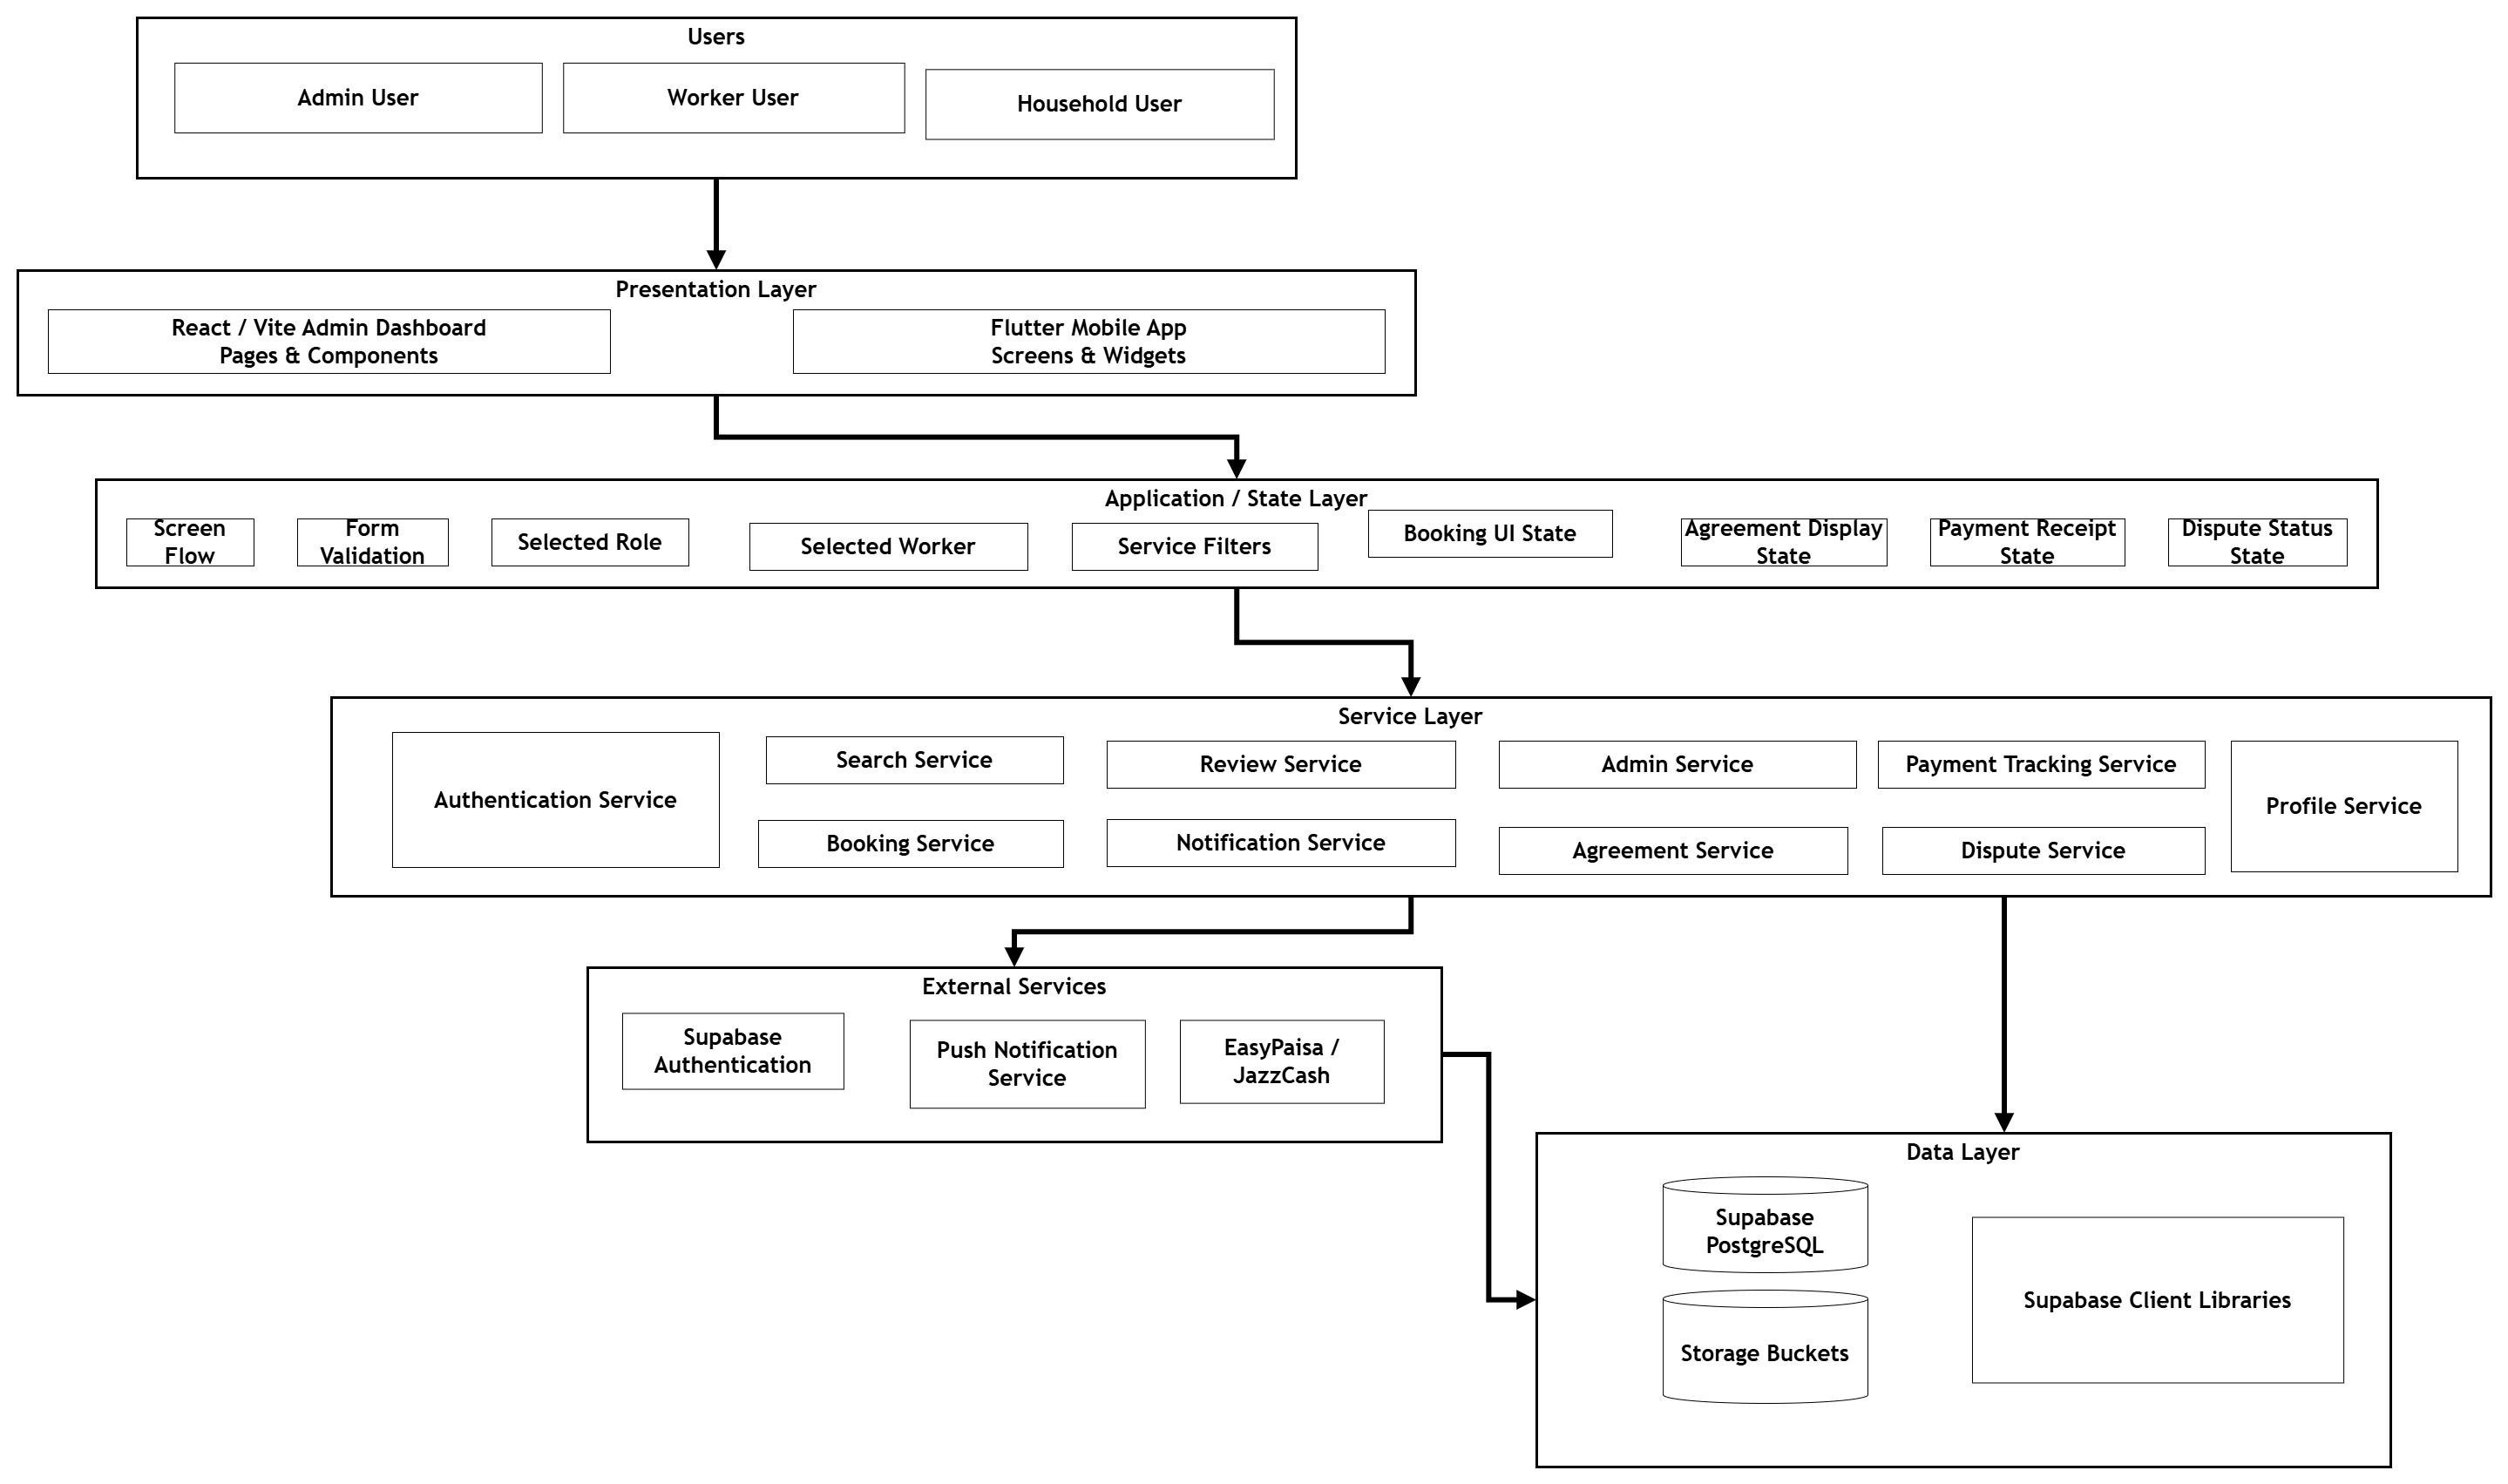
\includegraphics[width=0.95\linewidth,height=0.72\textheight,keepaspectratio]{thesis-assets/image3.png}
\caption{High-Level System Architecture of the HomeEase Platform}
\label{fig:architecture}
\end{figure}

\clearpage
\subsection{Process Flow Representation}
The platform orchestrates multi-step, multi-actor operational workflows across the booking, marketplace, recommendation, and verification cycles:

\begin{figure}[H]
\centering
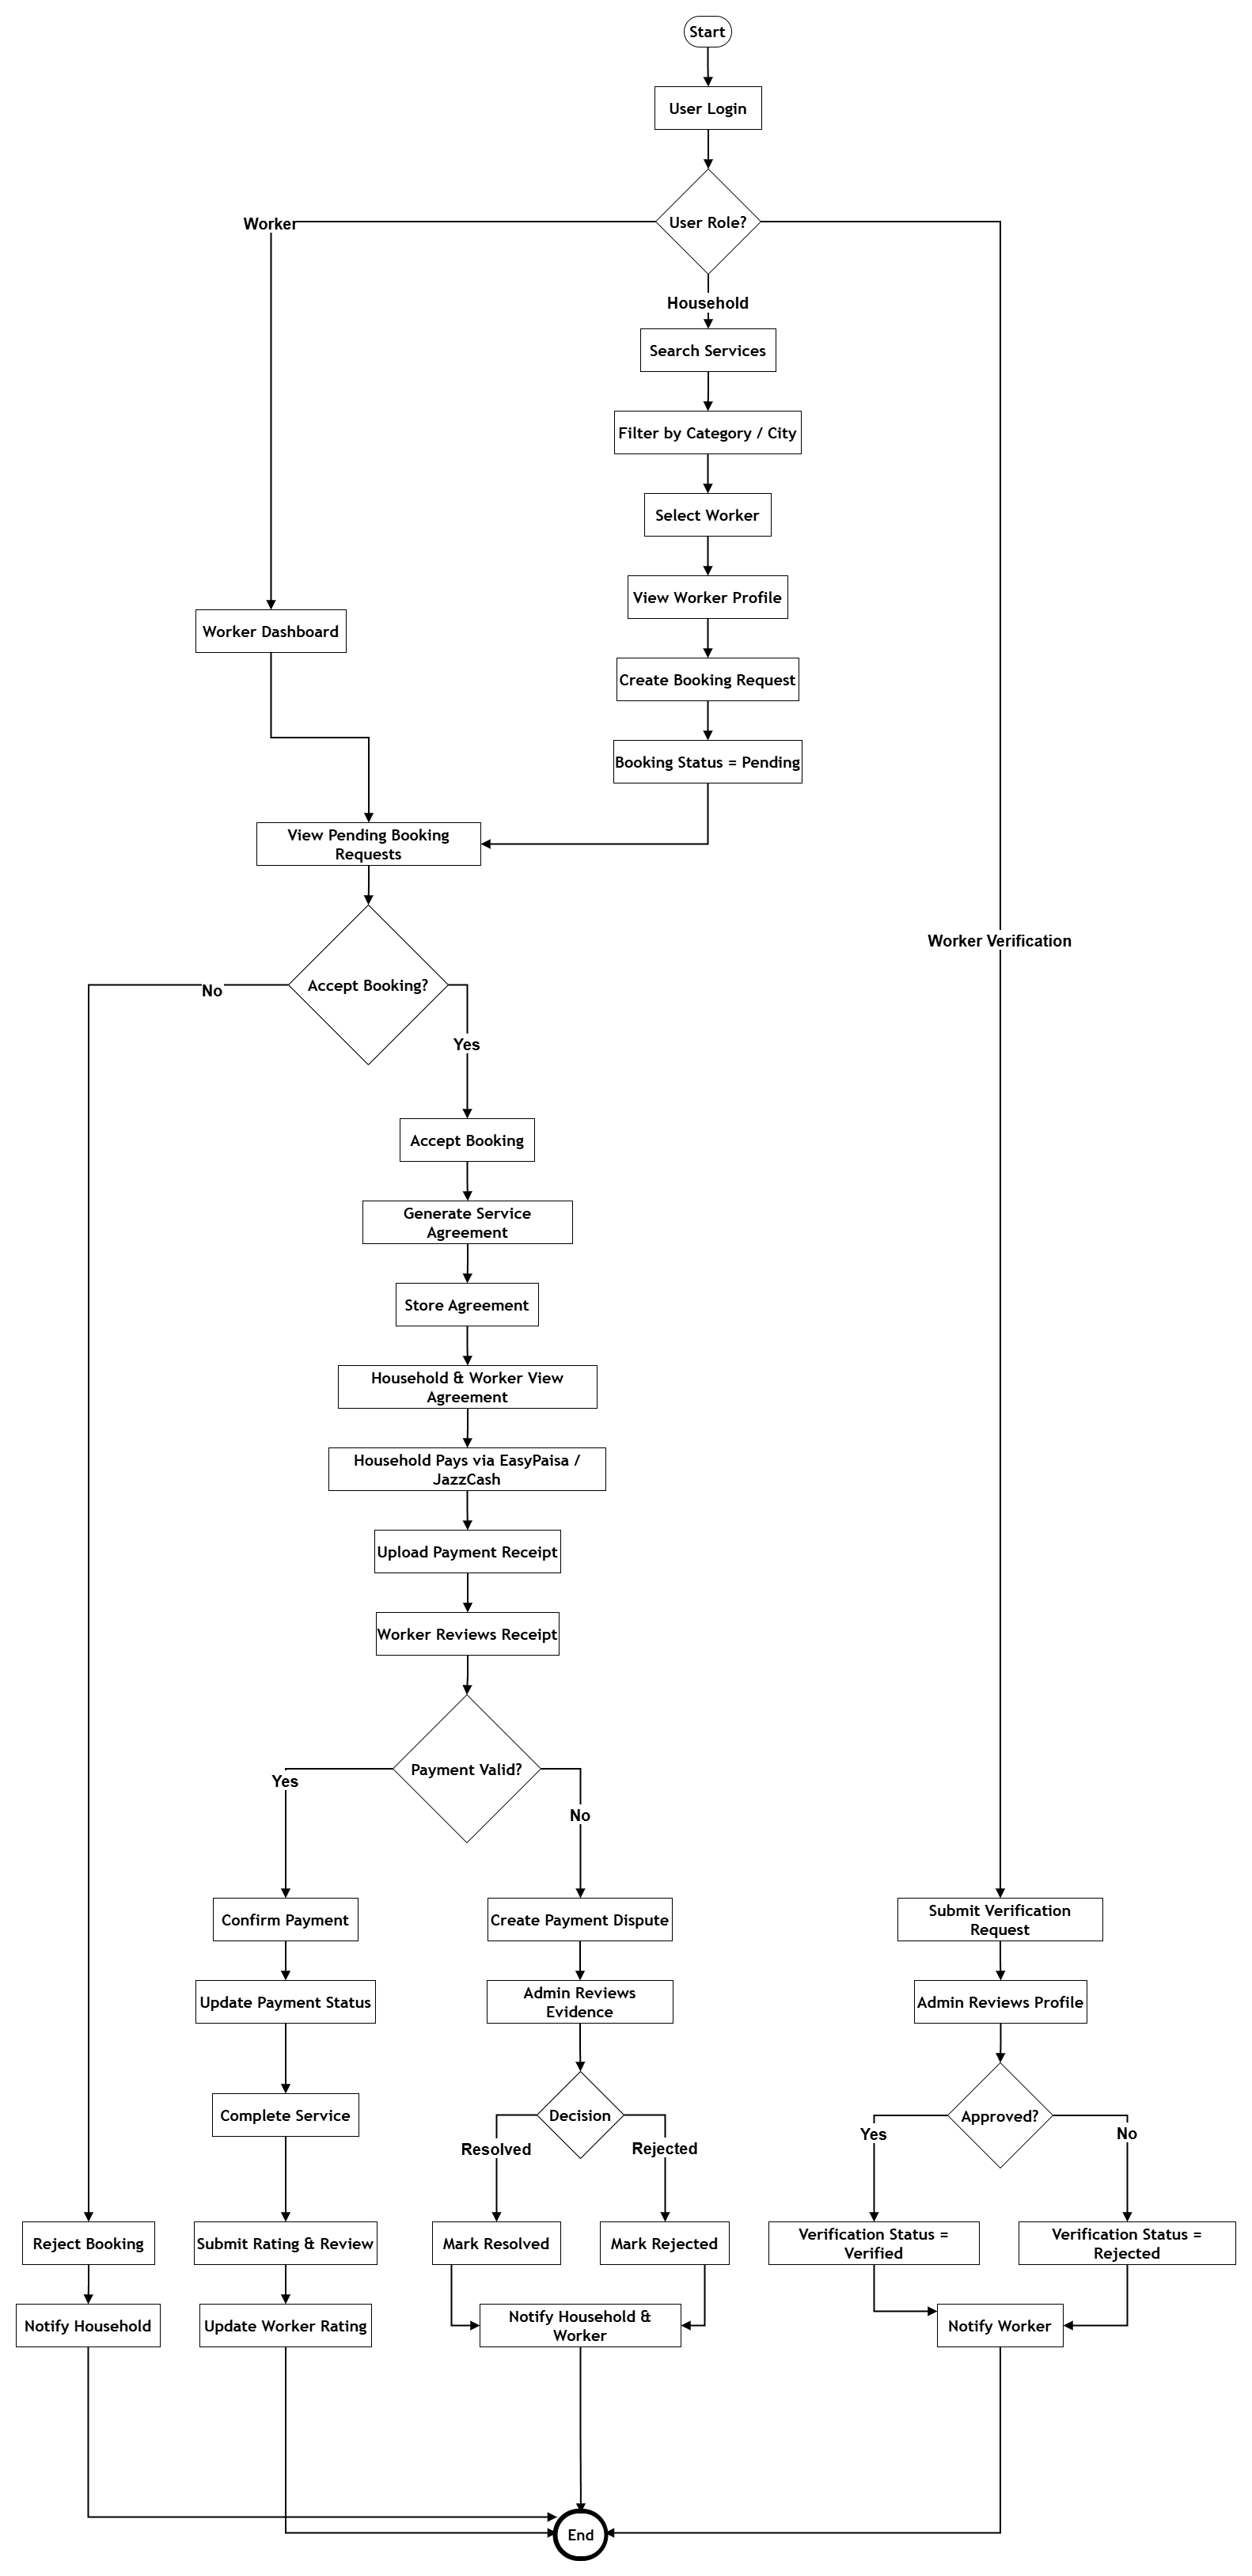
\includegraphics[width=0.95\linewidth,height=0.72\textheight,keepaspectratio]{thesis-assets/image4.png}
\caption{End-to-End Operational Process Flow in HomeEase}
\label{fig:process-flow}
\end{figure}

\clearpage
\subsection{Design Models}
\subsubsection{Class Diagram}
The object-oriented design model encapsulates the system domain into cohesive entity and service classes:

\begin{figure}[H]
\centering
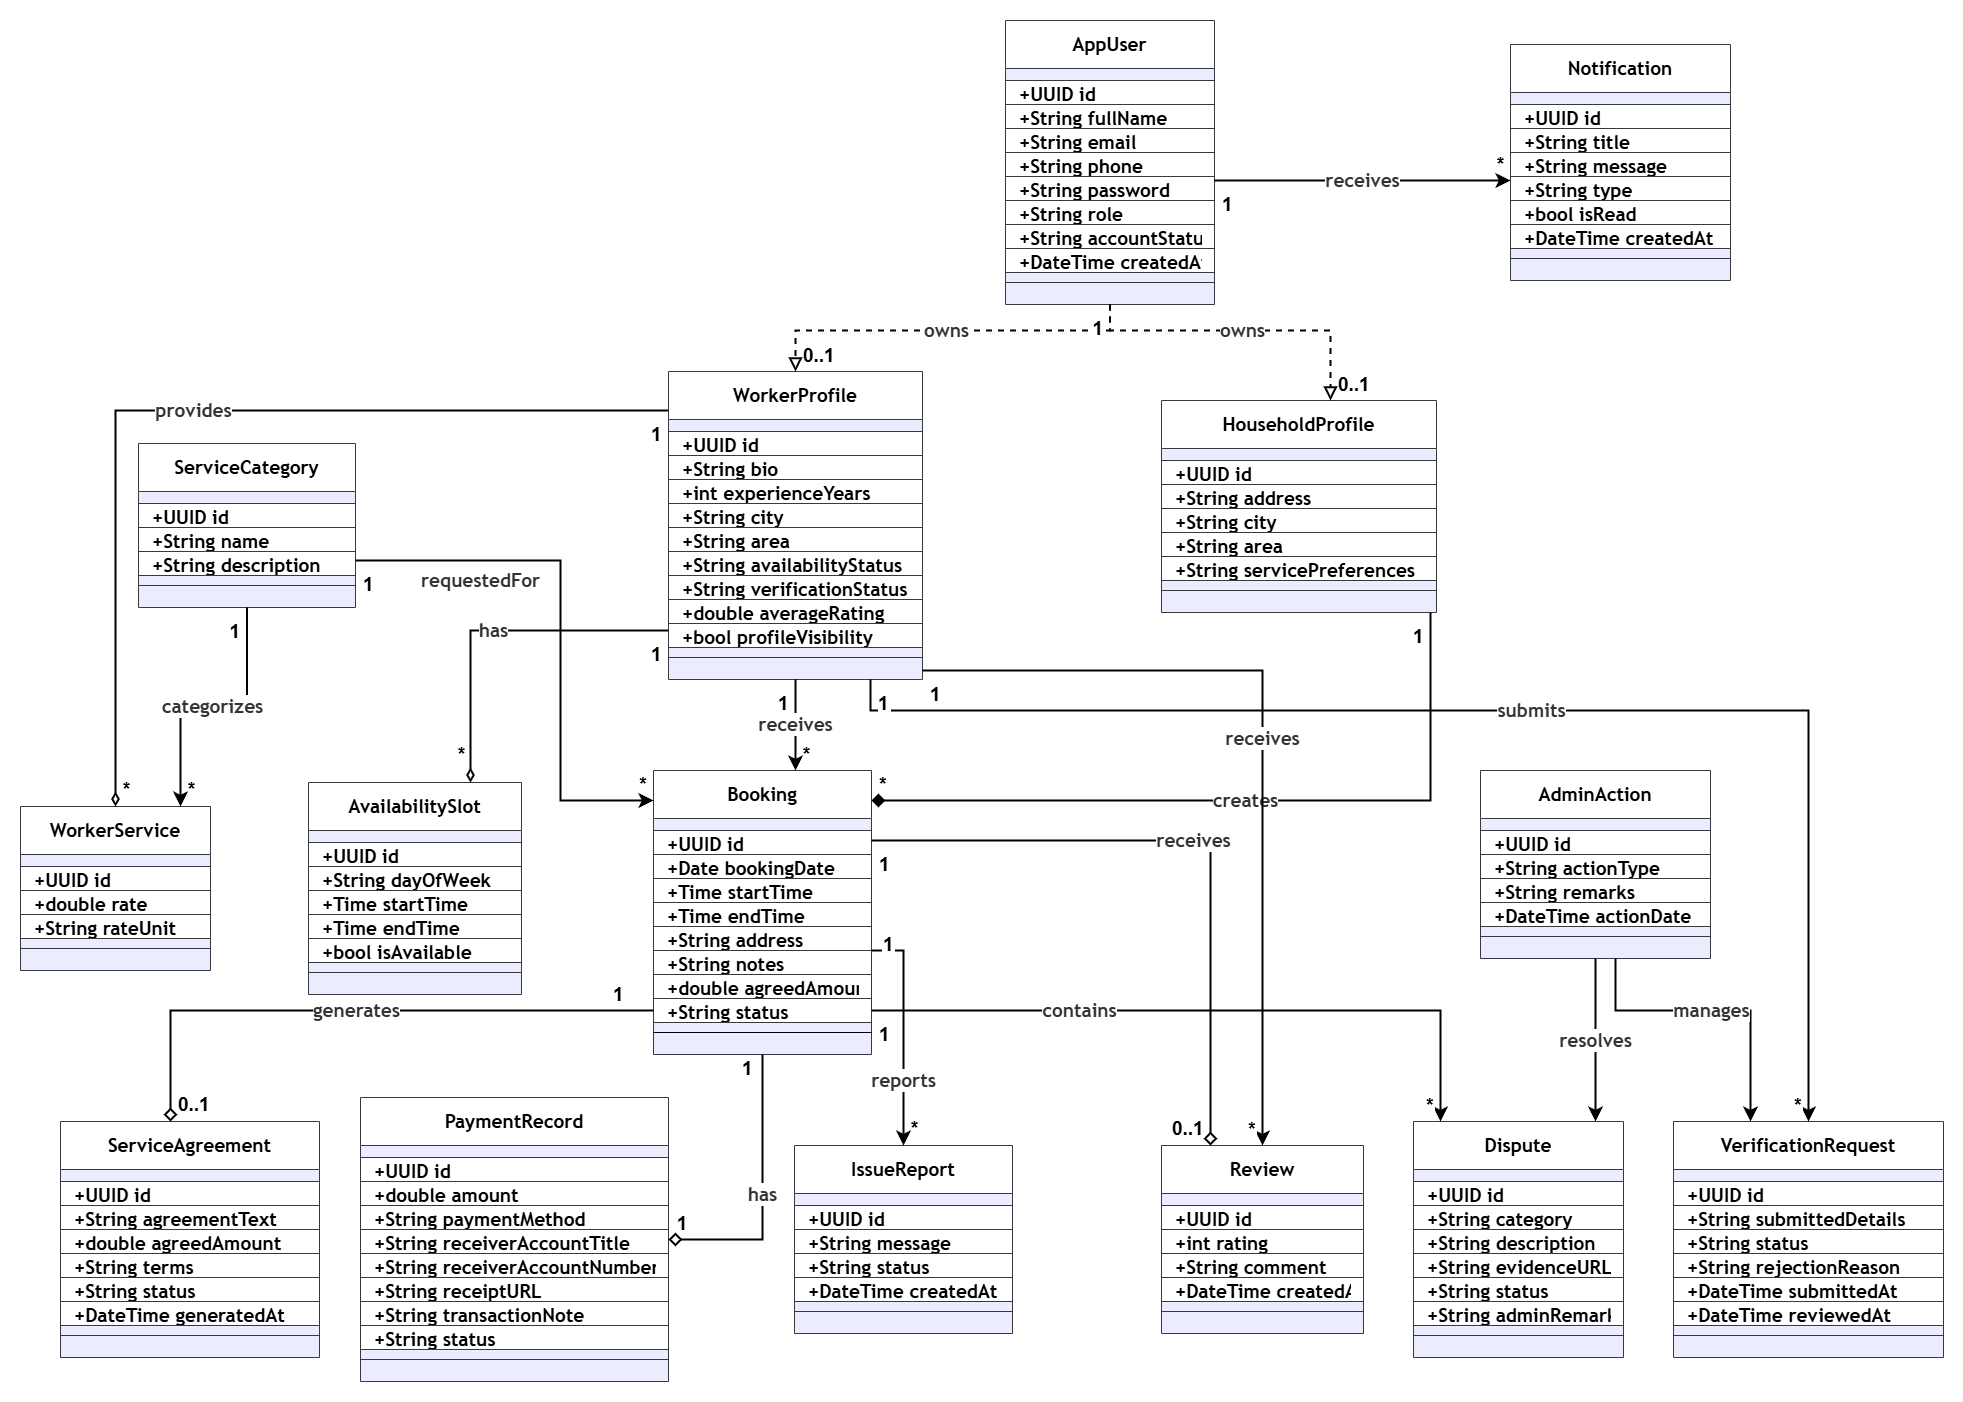
\includegraphics[width=0.95\linewidth,height=0.72\textheight,keepaspectratio]{thesis-assets/image5.png}
\caption{Class Diagram of HomeEase Core Domain Models}
\label{fig:class-diagram}
\end{figure}

\clearpage
\subsubsection{Sequence Diagram}
The sequence model formalizes dynamic message passing between user interfaces, controllers, recommendation engines, and database services during the AI Search, Booking Request, and Job Application lifecycles.

\begin{figure}[H]
\centering
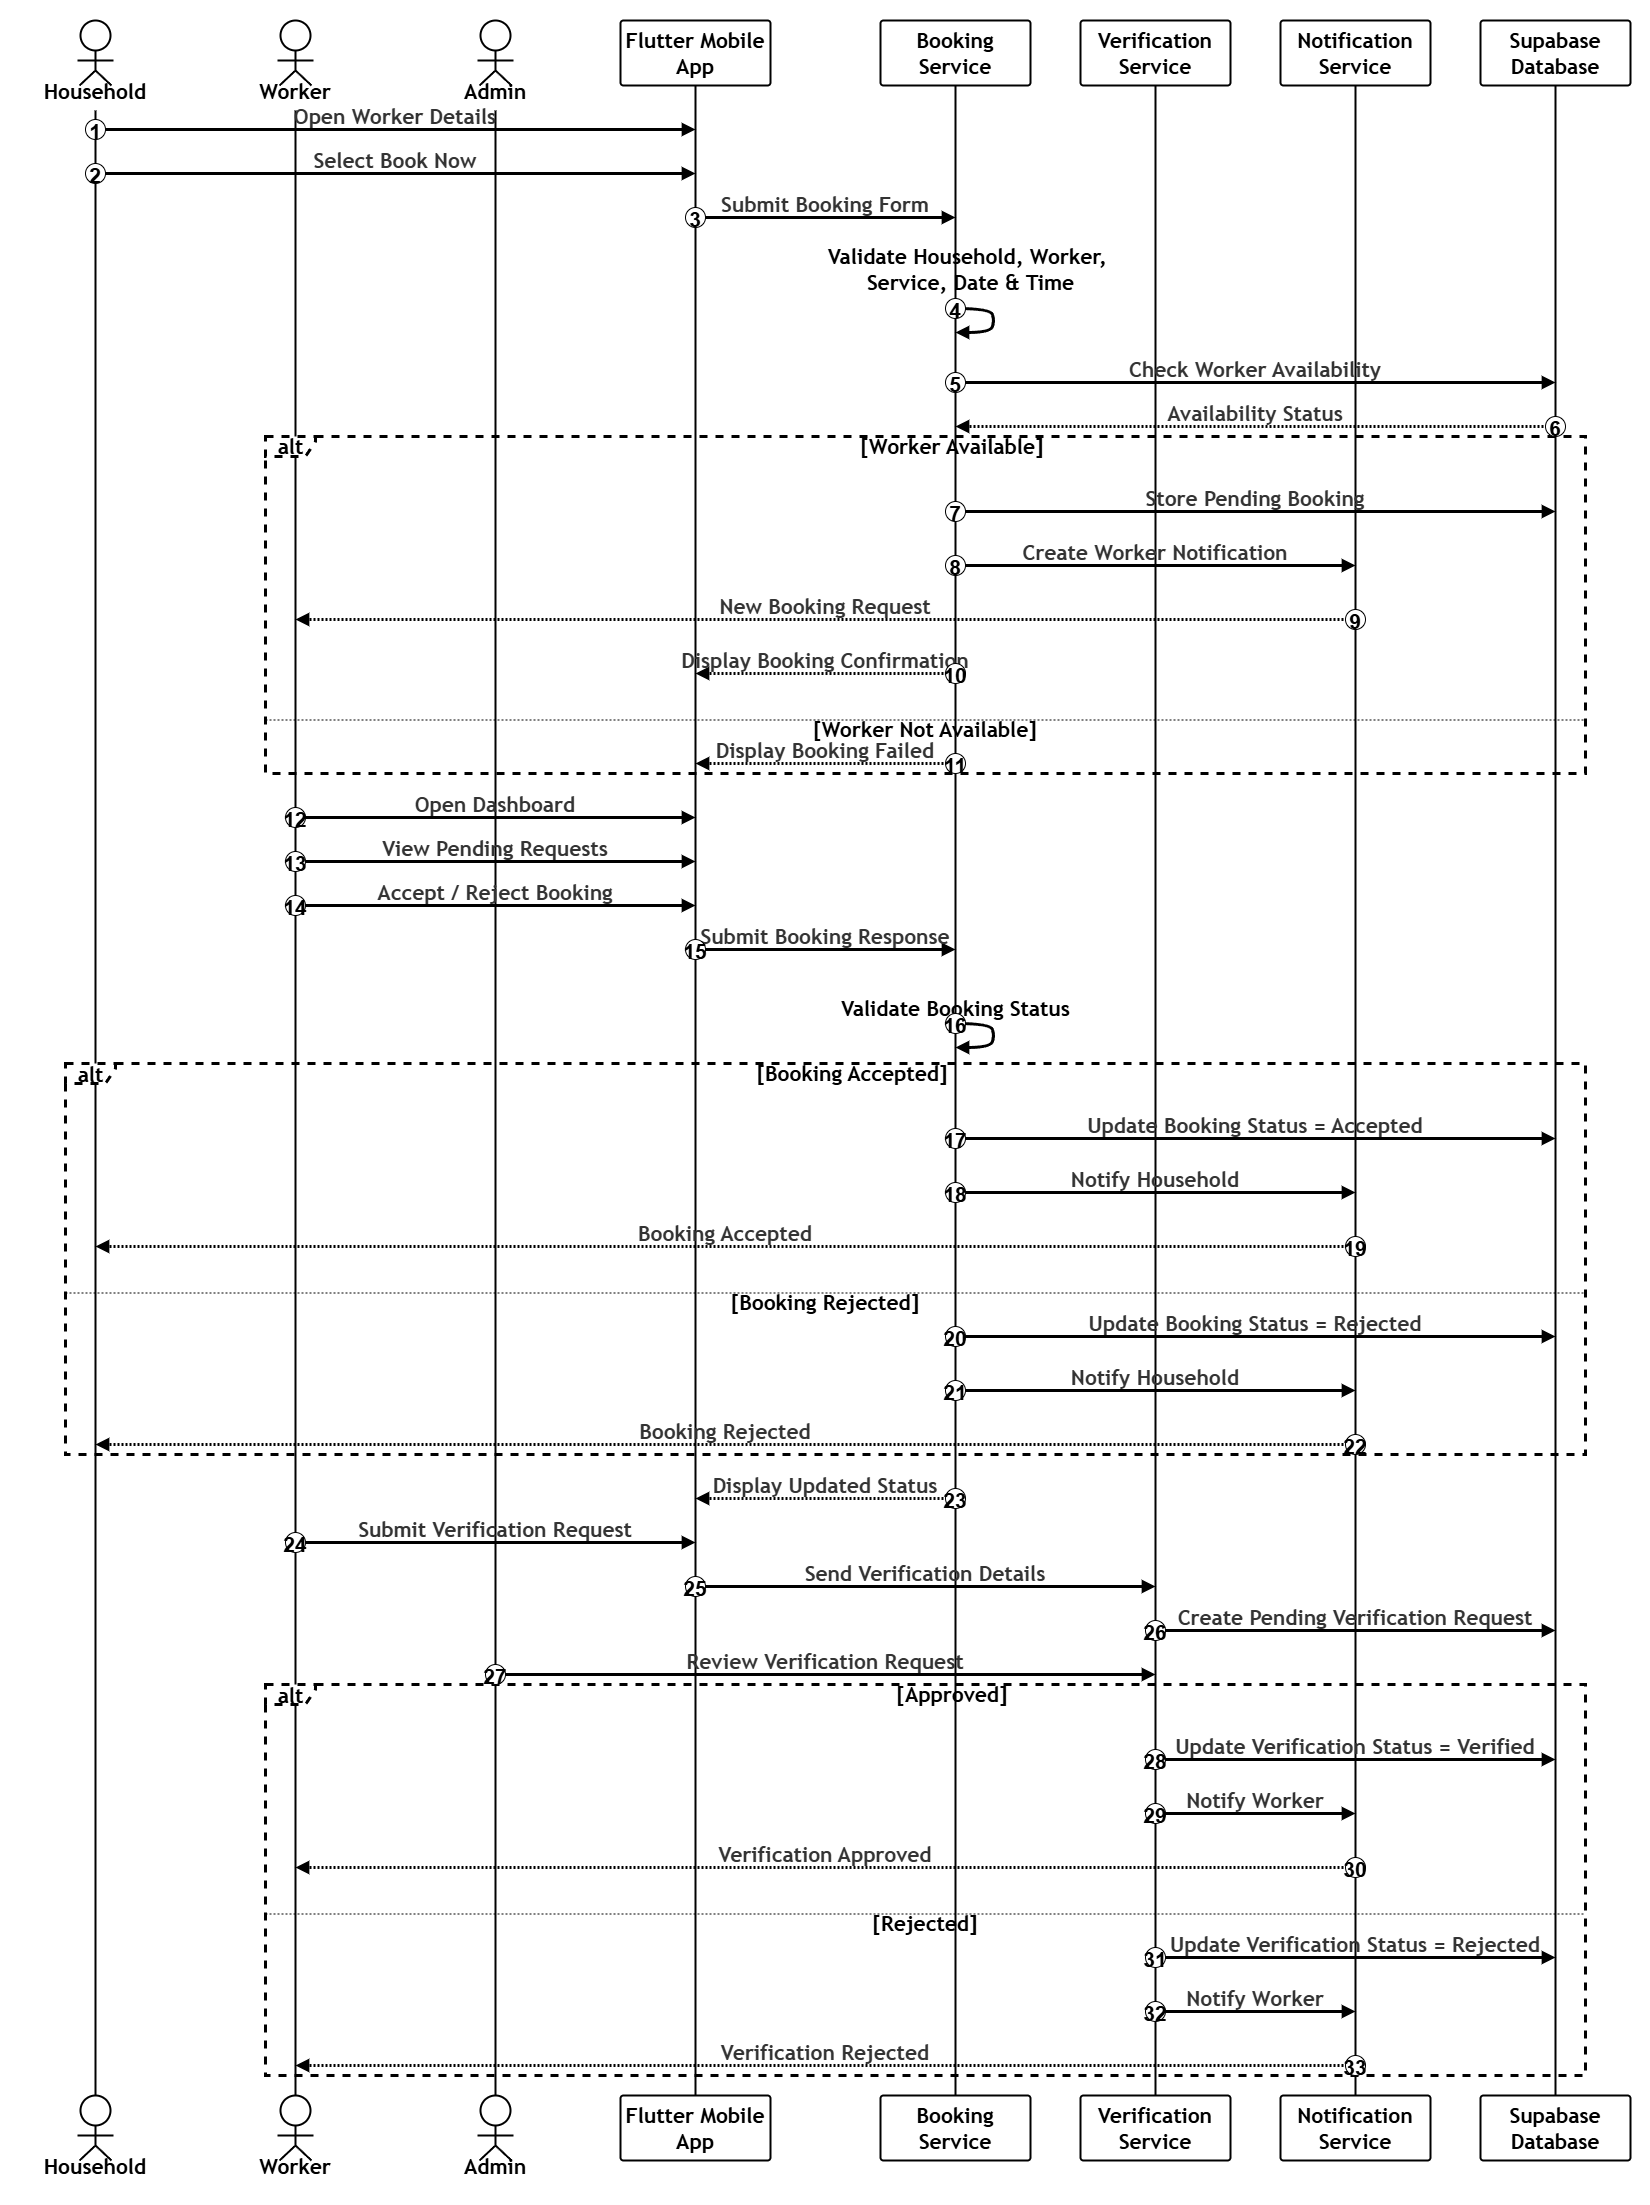
\includegraphics[width=0.95\linewidth,height=0.72\textheight,keepaspectratio]{thesis-assets/image6.png}
\caption{Sequence Diagram for AI Recommendation and Booking Lifecycle}
\label{fig:sequence-diagram}
\end{figure}

\clearpage
\subsubsection{State Transition Model}
HomeEase coordinates several critical state machines:

\begin{figure}[H]
\centering
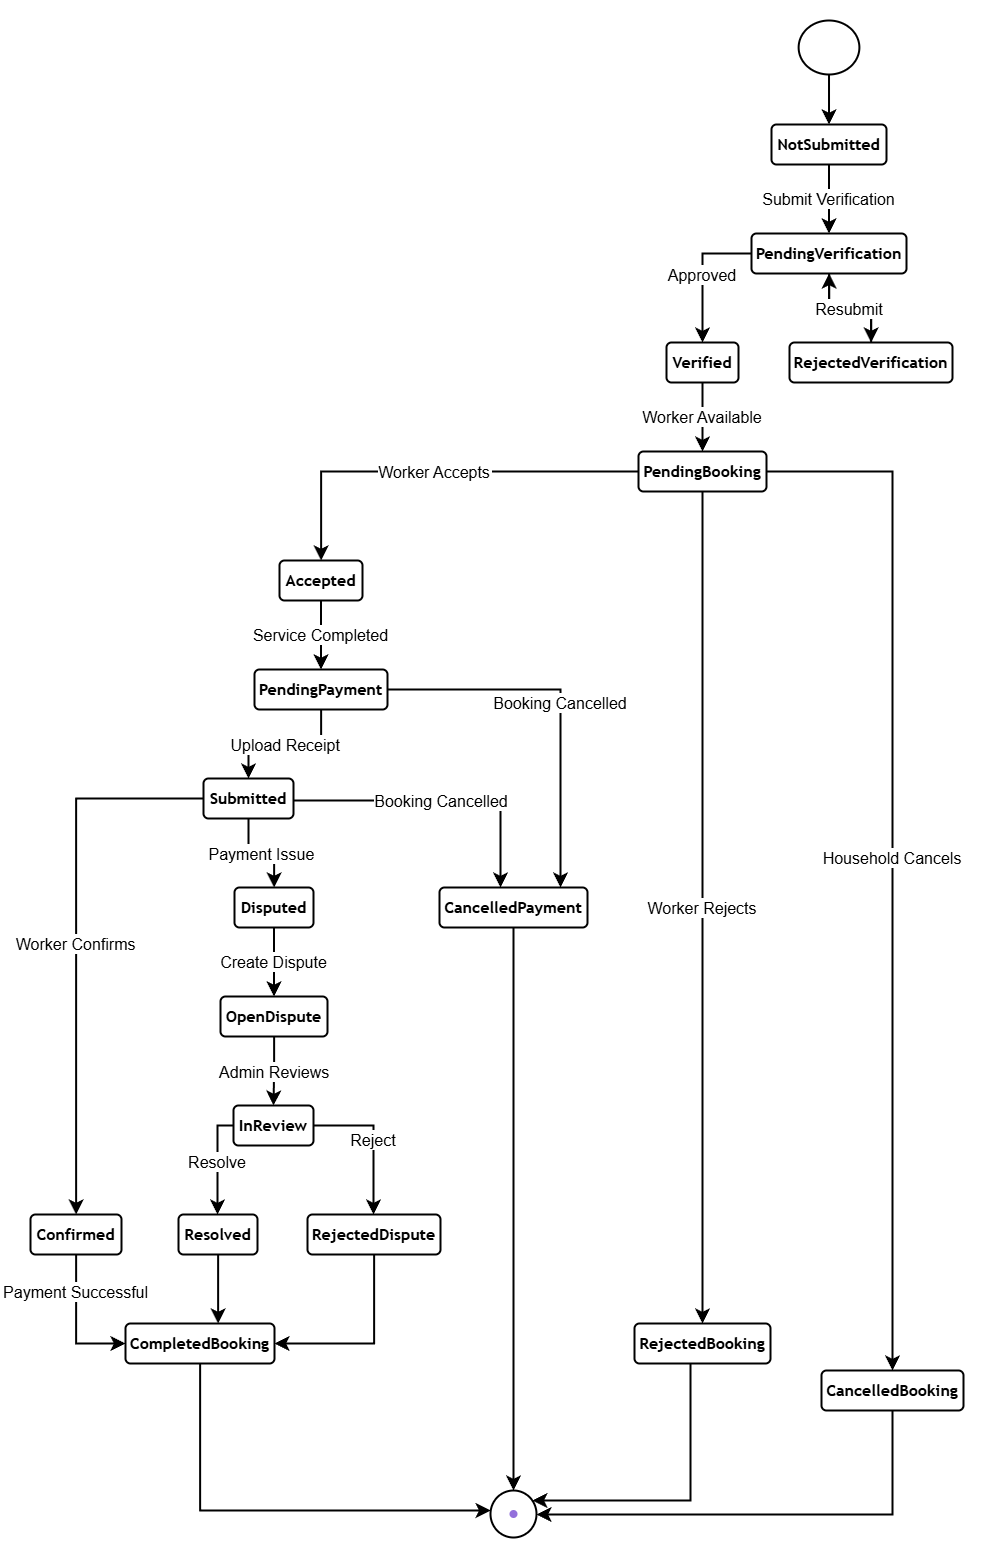
\includegraphics[width=0.95\linewidth,height=0.72\textheight,keepaspectratio]{thesis-assets/image7.png}
\caption{State Transition Diagram for Booking, Job Post, and Verification Lifecycles}
\label{fig:state-transition}
\end{figure}

\clearpage
\subsubsection{Entity-Relationship Diagram \& Data Dictionary}
The relational database schema is modeled in PostgreSQL and normalized to Third Normal Form (3NF). It comprises 16 relational tables:

\begin{figure}[H]
\centering
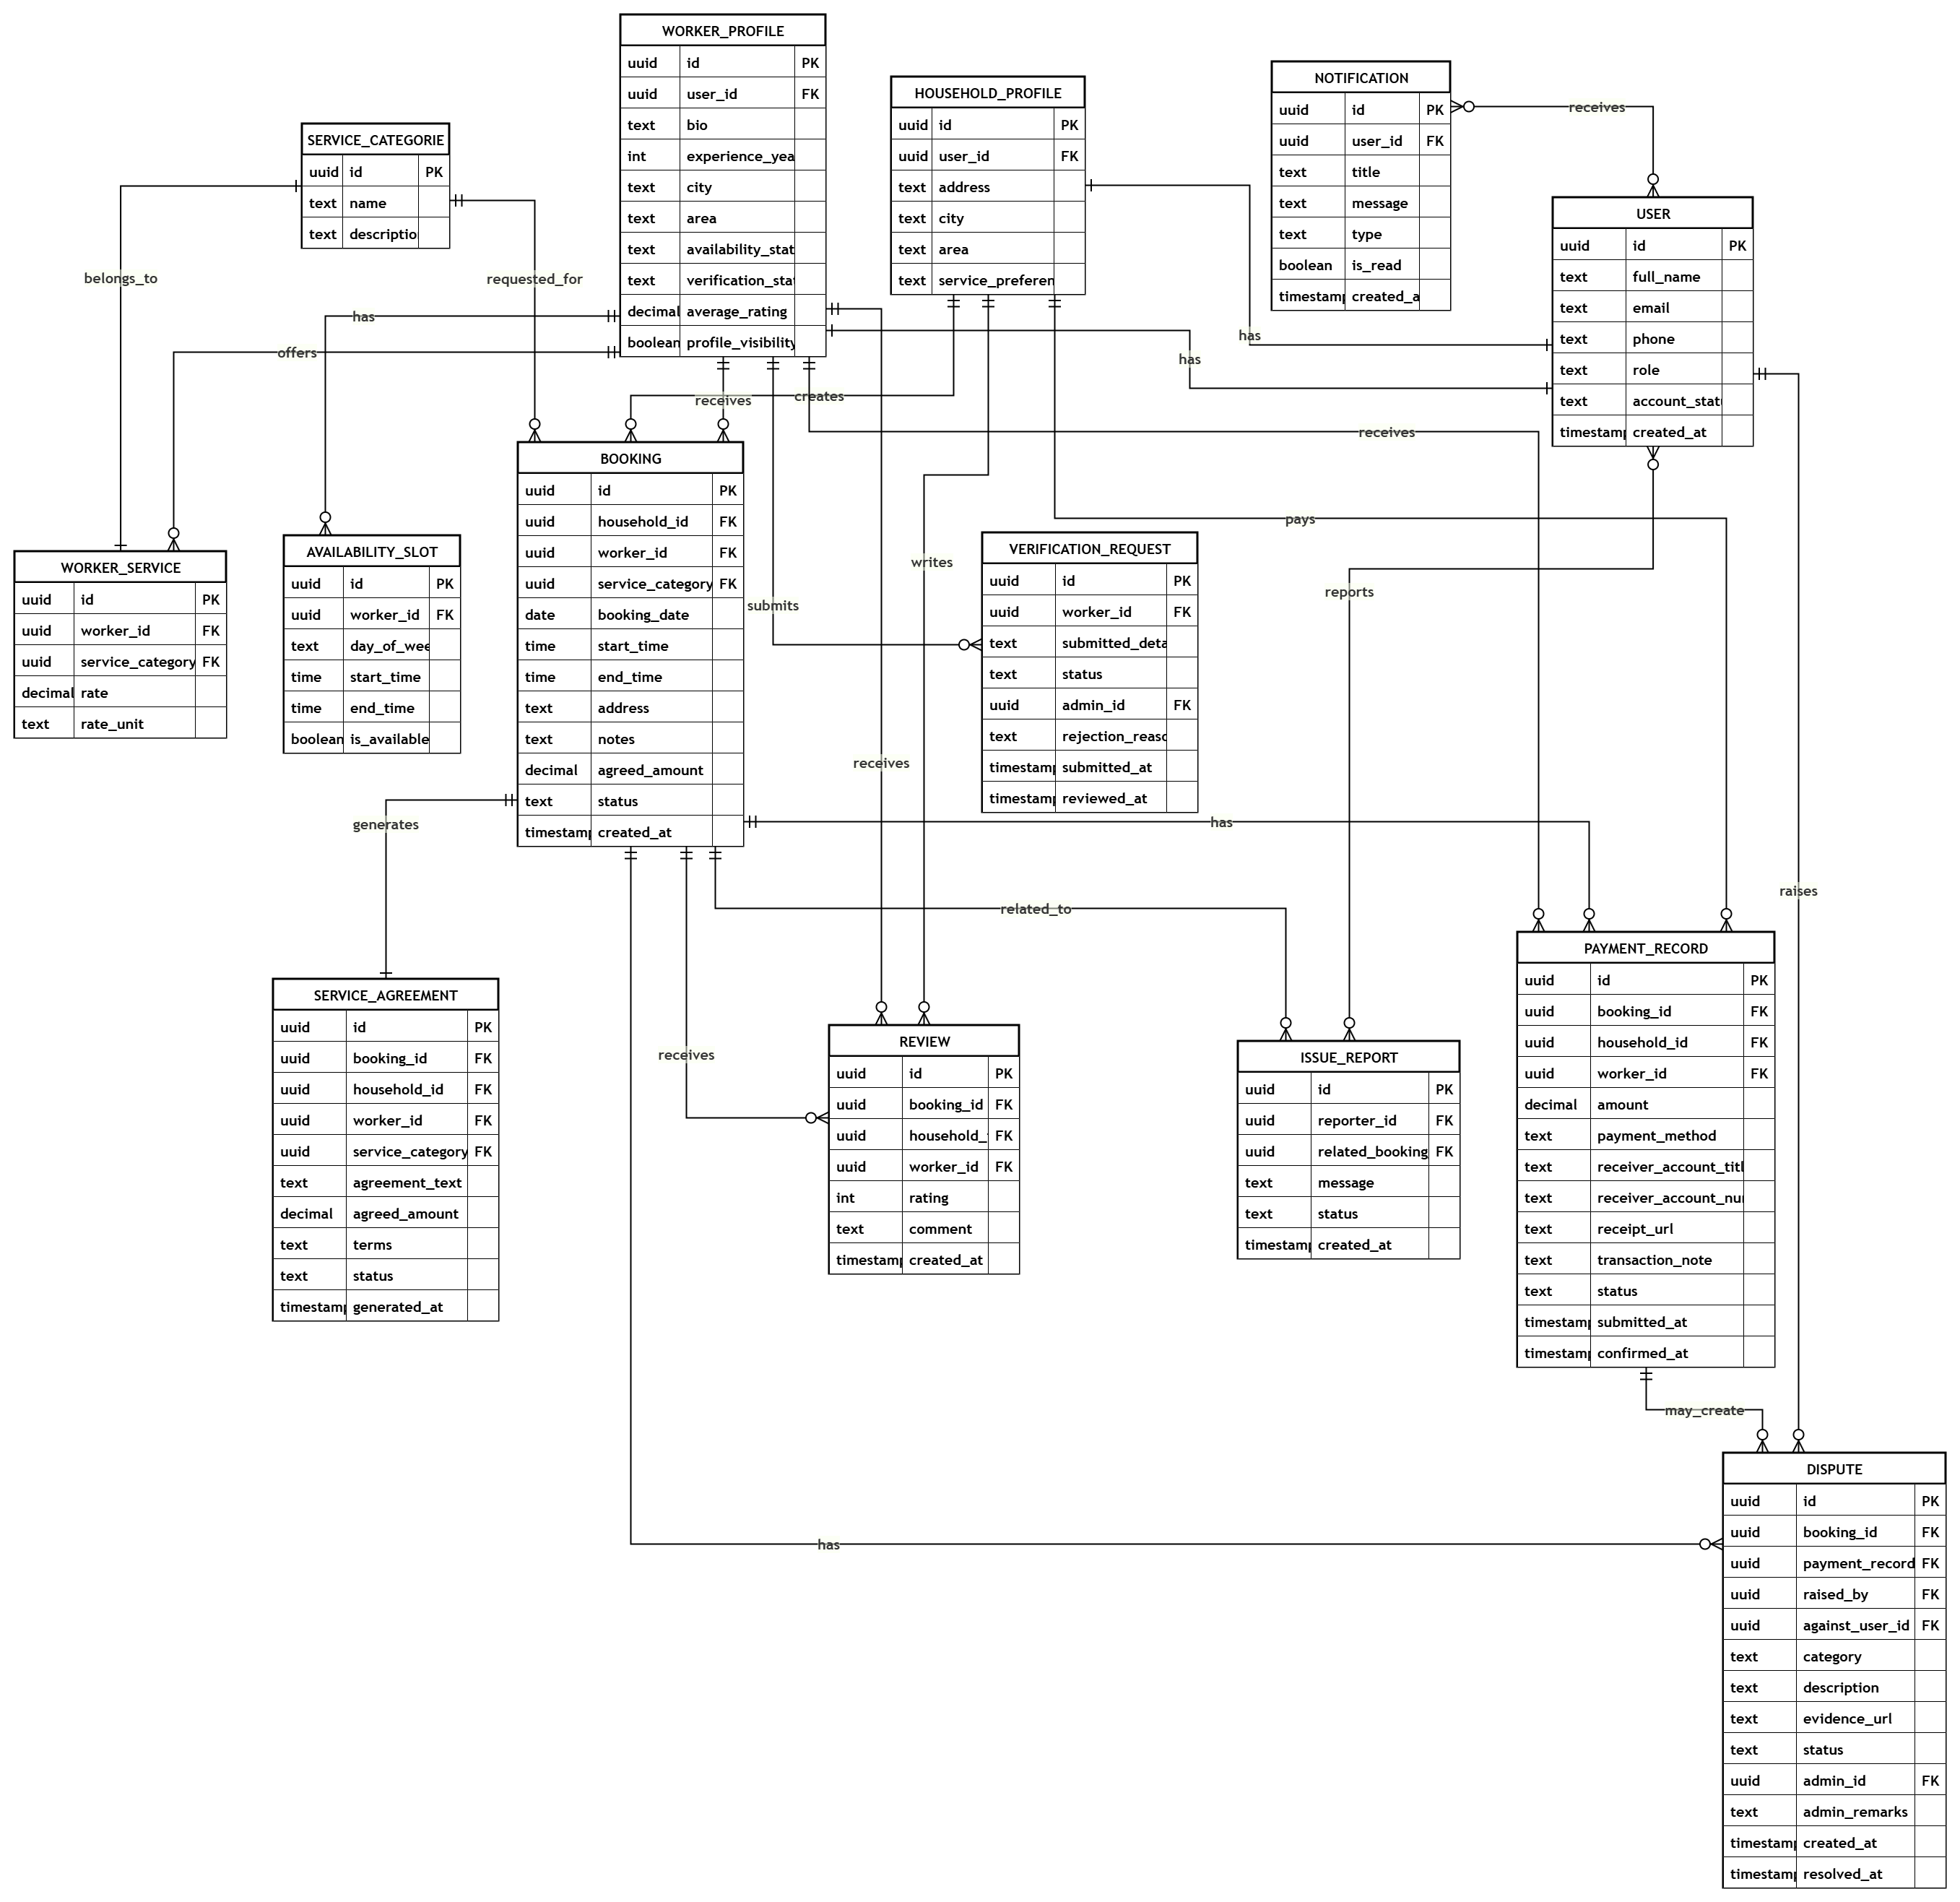
\includegraphics[width=0.95\linewidth,height=0.72\textheight,keepaspectratio]{thesis-assets/image8.png}
\caption{Entity-Relationship Diagram of the HomeEase PostgreSQL Database}
\label{fig:erd}
\end{figure}

Data Dictionary Table Overview:

\begingroup
\setstretch{1}
\fontsize{10}{11.5}\selectfont
\setlength{\tabcolsep}{4pt}
\setlength{\extrarowheight}{2pt}
\setlength{\LTpre}{6pt}
\setlength{\LTpost}{10pt}
\begin{longtable}{|>{\bfseries\raggedright\arraybackslash}p{\dimexpr(\linewidth-8\tabcolsep-5\arrayrulewidth)/4\relax}|>{\raggedright\arraybackslash}p{\dimexpr(\linewidth-8\tabcolsep-5\arrayrulewidth)/4\relax}|>{\raggedright\arraybackslash}p{\dimexpr(\linewidth-8\tabcolsep-5\arrayrulewidth)/4\relax}|>{\raggedright\arraybackslash}p{\dimexpr(\linewidth-8\tabcolsep-5\arrayrulewidth)/4\relax}|}
\caption{HomeEase Database Data Dictionary}\label{tab:data-dictionary}\\
\hline
\textbf{Table Name} & \textbf{Primary Key} & \textbf{Foreign Keys} & \textbf{Functional Purpose} \\ \hline
\endfirsthead
\multicolumn{4}{c}{Table \thetable\ HomeEase Database Data Dictionary (continued)}\\
\hline
\textbf{Table Name} & \textbf{Primary Key} & \textbf{Foreign Keys} & \textbf{Functional Purpose} \\ \hline
\endhead
\endfoot
\endlastfoot
USERS & id (UUID) & None & Master account records, email, phone, role, password hash, account status. \\ \hline
HOUSEHOLD\_\allowbreak{}PROFILES & id (UUID) & user\_\allowbreak{}id -> USERS(id) & Household employer profile, Abbottabad address, locality, preferred language. \\ \hline
WORKER\_\allowbreak{}PROFILES & id (UUID) & user\_\allowbreak{}id -> USERS(id) & Worker profile, experience years, bio, latitude, longitude, verified flag, rating. \\ \hline
SERVICE\_\allowbreak{}CATEGORIES & id (UUID) & None & Service classifications (Cooking, Cleaning, Childcare, Elderly Care, Maid). \\ \hline
WORKER\_\allowbreak{}SERVICES & id (UUID) & worker\_\allowbreak{}id, category\_\allowbreak{}id & Associative table mapping worker specializations with hourly/\allowbreak{}visit rates. \\ \hline
AVAILABILITY\_\allowbreak{}SLOTS & id (UUID) & worker\_\allowbreak{}id -> WORKER\_\allowbreak{}PROFILES(id) & Weekly day-of-week worker availability intervals and active toggles. \\ \hline
BOOKINGS & id (UUID) & household\_\allowbreak{}id, worker\_\allowbreak{}id, category\_\allowbreak{}id & Central transactional entity linking employer, worker, date, hours, and status. \\ \hline
SERVICE\_\allowbreak{}AGREEMENTS & id (UUID) & booking\_\allowbreak{}id, household\_\allowbreak{}id, worker\_\allowbreak{}id & Auto-generated formal service contract text, agreed fee, and signing status. \\ \hline
JOB\_\allowbreak{}POSTS & id (UUID) & household\_\allowbreak{}id, category\_\allowbreak{}id & Bidirectional marketplace open gig listings with budget, locality, and date. \\ \hline
JOB\_\allowbreak{}APPLICATIONS & id (UUID) & job\_\allowbreak{}post\_\allowbreak{}id, worker\_\allowbreak{}id & Worker applications submitted against open gigs with proposed rates. \\ \hline
PAYMENT\_\allowbreak{}RECORDS & id (UUID) & booking\_\allowbreak{}id, household\_\allowbreak{}id, worker\_\allowbreak{}id & Manual payment audit records (Cash/\allowbreak{}JazzCash/\allowbreak{}EasyPaisa), receipt URLs, confirmation. \\ \hline
REVIEWS & id (UUID) & booking\_\allowbreak{}id, household\_\allowbreak{}id, worker\_\allowbreak{}id & Multi-factor ratings (punctuality, behavior, quality) and written comments. \\ \hline
VERIFICATION\_\allowbreak{}REQUESTS & id (UUID) & worker\_\allowbreak{}id, admin\_\allowbreak{}id & KYC audit submissions containing CNIC front/\allowbreak{}back URLs and review remarks. \\ \hline
DISPUTES & id (UUID) & booking\_\allowbreak{}id, raised\_\allowbreak{}by, admin\_\allowbreak{}id & Transaction grievances, evidence URLs, mediation status, and admin resolution. \\ \hline
NOTIFICATIONS & id (UUID) & user\_\allowbreak{}id -> USERS(id) & In-app and push notification alerts for booking status and gig updates. \\ \hline
ISSUE\_\allowbreak{}REPORTS & id (UUID) & reporter\_\allowbreak{}id, booking\_\allowbreak{}id & General platform feedback, technical bug reports, and safety alerts. \\ \hline
\end{longtable}
\endgroup
\clearpage\section{References}
\begin{list}{}{\setlength{\leftmargin}{0pt}\setlength{\itemindent}{0pt}\setlength{\itemsep}{6pt}\setlength{\parsep}{0pt}}
\item Sommerville, I. (2016). \textit{Software Engineering} (10th ed.). Pearson Education.
\item Pressman, R. S., \& Maxim, B. R. (2020). \textit{Software Engineering: A Practitioner's Approach} (9th ed.). McGraw-Hill Education.
\item Ricci, F., Rokach, L., \& Shapira, B. (2022). \textit{Recommender Systems Handbook} (3rd ed.). Springer US.
\item Sinnott, R. W. (1984). Virtues of the Haversine. \textit{Sky and Telescope}, 68(2), 159.
\item Nielsen, J. (1994). \textit{Usability Engineering}. Morgan Kaufmann Publishers.
\item Medhi, I., Sagar, A., \& Toyama, K. (2007). Text-Free User Interfaces for Illiterate and Semi-Literate Users. \textit{Information Technologies and International Development}, 4(1), 37--50.
\item Google. (2024). Flutter Documentation: Architectural Overview and Reactive State. \url{https://docs.flutter.dev/}
\item Supabase Inc. (2024). Supabase PostgreSQL \& Row Level Security Architecture Guide. \url{https://supabase.com/docs/}
\item International Labour Organization. (2021). \textit{Making Decent Work a Reality for Domestic Workers}. Geneva: ILO.
\item Pakistan Bureau of Statistics. (2022). \textit{Labour Force Survey 2020--21}. Government of Pakistan.
\item Salton, G., \& McGill, M. J. (1983). \textit{Introduction to Modern Information Retrieval}. McGraw-Hill.
\item Pazzani, M. J., \& Billsus, D. (2007). Content-Based Recommendation Systems. In \textit{The Adaptive Web} (pp. 325--341). Springer.
\item Lundberg, S. M., \& Lee, S. I. (2017). A Unified Approach to Interpreting Model Predictions. \textit{Advances in Neural Information Processing Systems}, 30.
\item Fielding, R. T. (2000). \textit{Architectural Styles and the Design of Network-Based Software Architectures}. Doctoral dissertation, University of California, Irvine.
\item ISO/IEC/IEEE. (2017). \textit{Systems and Software Engineering---Architecture Description}. ISO/IEC/IEEE 42010 standard.
\item World Bank. (2023). \textit{Pakistan Digital Economy Assessment: Unleashing Inclusive Growth}. Washington, DC: World Bank.
\end{list}

\end{document}